\documentclass[12pt,a4paper]{report}

% --- Pacotes Fundamentais ---
\usepackage[utf8]{inputenc}
\usepackage[T1]{fontenc}
\usepackage[brazil]{babel}
\usepackage{amsmath,amsfonts,amssymb}
\usepackage{graphicx}
\usepackage{booktabs}
\usepackage{microtype}
\usepackage{url}
\usepackage{cite}
\usepackage{float}
\usepackage{titlesec}
\usepackage{caption}

% --- Geometria e Formatação ABNT ---
\usepackage[a4paper, top=3cm, bottom=2cm, left=3cm, right=2cm]{geometry}
\usepackage{setspace}
\onehalfspacing
\usepackage{indentfirst}
\setlength{\parindent}{1.25cm}
\graphicspath{ {./images/} }

% --- Configurações de Hiperlinks ---
\usepackage[colorlinks=true,
            linkcolor=blue,
            citecolor=blue,
            urlcolor=blue,
            bookmarks=true]{hyperref}

% --- Ajuste dos Títulos de Capítulos e Seções ---
\titleformat{\chapter}[hang]
  {\normalfont\bfseries\LARGE}{\thechapter}{1em}{}
\titlespacing*{\chapter}{0pt}{-20pt}{20pt}

\titleformat{\section}[hang]
  {\normalfont\bfseries\Large}{\thesection}{1em}{}
\titlespacing*{\section}{0pt}{15pt}{10pt}

\titleformat{\subsection}[hang]
  {\normalfont\bfseries\large}{\thesubsection}{1em}{}
\titlespacing*{\subsection}{0pt}{12pt}{8pt}

\begin{document}

% -----------------------------------------------------------------------------
% ELEMENTOS PRÉ-TEXTUAIS: CAPA E FOLHA DE ROSTO
% -----------------------------------------------------------------------------
\begin{titlepage}
    \centering
    \vspace*{1cm}
    {\large \textbf{JUAN AUGUSTO CRISTO HYGINO}\par}
    \vspace{6cm}
    {\LARGE \textbf{ENGENHARIA DE UMA CAMADA DE GOVERNANÇA, AUDITORIA FORENSE E OBSERVABILIDADE EM TEMPO DE EXECUÇÃO PARA ECOSSISTEMAS BASEADOS NO MODEL CONTEXT PROTOCOL (MCP)}\par}
    \vfill
    {\large \textbf{2026}\par}
    \vspace*{1cm}
\end{titlepage}

 \begin{titlepage}
     \centering
     \vspace*{1cm}
     {\large \textbf{JUAN AUGUSTO CRISTO HYGINO}\par}
     \vspace{4.5cm}
     {\LARGE \textbf{ENGENHARIA DE UMA CAMADA DE GOVERNANÇA, AUDITORIA FORENSE E OBSERVABILIDADE EM TEMPO DE EXECUÇÃO PARA ECOSSISTEMAS BASEADOS NO MODEL CONTEXT PROTOCOL (MCP)}\par}
     \vspace{2.5cm}
     \hfill
     \begin{minipage}{0.52\textwidth}
         \linespread{1.1}\selectfont
         Trabalho de Conclusão de Curso submetido como requisito parcial para a obtenção do grau de Bacharel em Ciência da Computação / Engenharia de Software.\\[0.4cm]
         \textbf{Orientador:} Profa. Dra. Annabel D.R. Tamariz
     \end{minipage}
     \vfill
     {\large \textbf{2026}\par}
     \vspace*{1cm}
 \end{titlepage}

% --- Sumário ---
\tableofcontents
\thispagestyle{empty}
\clearpage

% Reinicia numeração para o corpo textual
\pagenumbering{arabic}
\setcounter{page}{1}

% -----------------------------------------------------------------------------
% ELEMENTOS TEXTUAIS: CAPÍTULO 1 - INTRODUÇÃO
% -----------------------------------------------------------------------------
\chapter{Introdução}
\label{cap:introducao}

A engenharia de software passa atualmente por uma profunda transformação com a transição dos Modelos de Linguagem de Larga Escala (\textit{Large Language Models} - LLMs) de interfaces conversacionais passivas para agentes autônomos orientados a objetivos. Diferente do modelo tradicional de perguntas e respostas pontuais, esses agentes operam em ciclos contínuos de raciocínio, planejamento e ação. Eles dividem metas complexas em etapas menores, definem parâmetros de execução e acionam rotinas em ambientes computacionais distribuídos \cite{buhler2026agentbound,singh2026mcpsecure}.

Para interagir com o mundo real e superar as limitações de seus dados de treinamento estáticos, os agentes de IA dependem do mecanismo de chamada de ferramentas (\textit{tool calling}) e do acesso a dados contextuais externos. Essas fontes incluem bancos de dados relacionais, sistemas de arquivos locais, repositórios de código e interfaces de programação de aplicações (APIs) \cite{zhu2025miniscope,hasan2026mcp}. No entanto, a integração entre modelos de linguagem e ferramentas externas sempre sofreu com a fragmentação técnica: cada plataforma adotava conectores proprietários e soluções pontuais, gerando forte acoplamento, problemas de compatibilidade e políticas de segurança frágeis ou inconsistentes.

Para resolver essa fragmentação, a Anthropic lançou no final de 2024 o \textit{Model Context Protocol} (MCP), uma arquitetura aberta de comunicação cliente-servidor baseada no protocolo JSON-RPC 2.0. O MCP rapidamente se consolidou como o padrão da indústria para conectar aplicações que hospedam modelos de IA (\textit{MCP Hosts/Clients}) a fontes de dados e ferramentas de execução (\textit{MCP Servers}) \cite{soriaparra2026mcp,hasan2026mcp}. Ao padronizar três conceitos fundamentais: ferramentas executáveis (\textit{tools}), dados e arquivos de leitura (\textit{resources}) e modelos de instrução (\textit{prompts}), o MCP permitiu que uma mesma aplicação cliente se conecte a dezenas de servidores locais (via canais de comunicação interprocessos \textit{stdio}) ou remotos (inicialmente via SSE e atualmente via \textit{Streamable HTTP}) \cite{soriaparra2026mcp}.


\begin{figure}[H]
  \centering
  \caption{Arquitetura de Integração do Model Context Protocol.}
  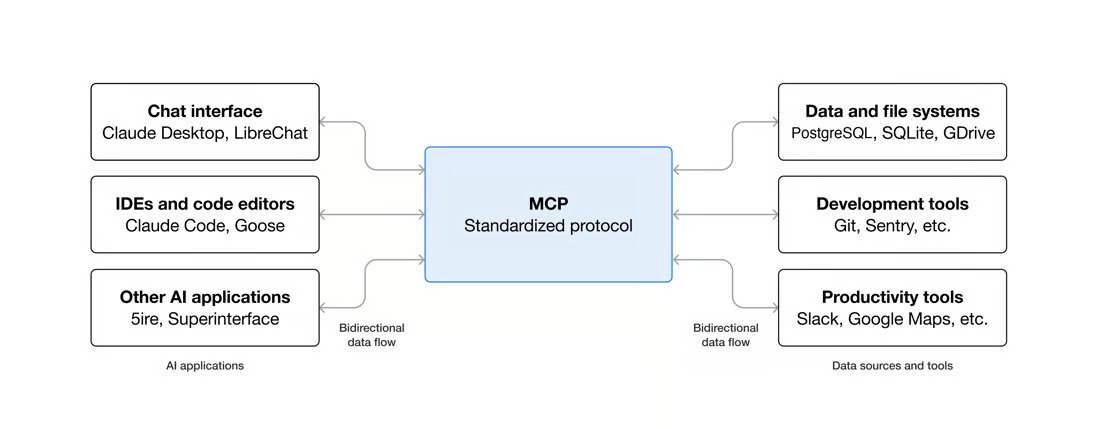
\includegraphics[scale=0.4]{mcp-official-anthropic-diagram.jpg}
  \label{fig:integration-arch}
  \caption*{Fonte: Anthropic (2024)}
\end{figure}

Apesar da facilidade de integração oferecida pelo protocolo, pesquisas recentes mostram que essa rápida expansão introduziu uma superfície de ataque ampla e preocupante no ecossistema de software \cite{guo2025measurement,hou2025mcp}. O MCP foi concebido sob uma postura estrutural de \textbf{confiança implícita}: uma vez realizada a conexão inicial entre o cliente e o servidor, o agente passa a ter acesso aberto a todas as ferramentas expostas, executando ações no sistema operacional com os mesmos privilégios do usuário logado \cite{buhler2026agentbound,singh2026mcpsecure}.

Estudos recentes de medição em larga escala comprovam a gravidade desse cenário. Em uma análise empírica de 1.899 servidores MCP de código aberto, Hasan et al. \cite{hasan2026mcp} identificaram que o protocolo apresenta uma superfície dual de ataque: além de 7,2\% dos servidores conterem falhas clássicas no código-fonte (com credenciais e chaves de acesso gravadas em texto simples em 3,6\% dos projetos), 5,5\% dos servidores já sofrem de envenenamento de ferramentas (\textit{Tool Poisoning}). Nesse tipo de ataque, descrições e esquemas das ferramentas são alterados de forma maliciosa para induzir o modelo de linguagem a tomar decisões incorretas ou prejudiciais, sem que o código executável precise ser modificado. Além disso, Guo et al. \cite{guo2025measurement} demonstraram que mais de 50\% dos servidores MCP em uso executam chamadas sensíveis no sistema hospedeiro (como execução de comandos de shell, leitura de arquivos e conexões de rede irrestritas) sem qualquer mecanismo de isolamento de processos.

Conforme analisado por Jang e Lee \cite{jang2026hierarchical}, o protocolo MCP funciona como um canal de integração que herda riscos de segurança em três camadas diferentes: na camada da própria LLM (injeções indiretas de prompt e alucinações), na camada do protocolo (ataques de intermediação maliciosa como \textit{Confused Deputy} e \textit{Puppet Attacks}) e na camada de infraestrutura de rede (envenenamento de DNS e ataques de atualização fraudulenta conhecidos como \textit{Rug Pull}, como o incidente registrado no servidor \texttt{postmark-mcp}).

Por outro lado, Bühler et al. \cite{buhler2026agentbound} destacaram a existência da \textbf{lacuna semântica} (\textit{Semantic Gap}) na segurança de agentes de IA: mecanismos tradicionais de isolamento do sistema operacional (como contêineres e políticas de controle de acesso de kernel) são essenciais para conter danos ao hospedeiro, mas não conseguem avaliar a intenção do agente nem impedir o uso indevido de ferramentas que tenham sido autorizadas no sistema. Ao mesmo tempo, Zhang et al. \cite{zhang2025acfix} comprovaram que confiar decisões de acesso à saída probabilística de modelos de linguagem gera falhas de quebra de controle de acesso (\textit{Broken Access Control}) em 47,4\% dos casos, reforçando a necessidade de aplicar modelos determinísticos de Controle de Acesso Baseado em Papéis (\textit{Role-Based Access Control} - RBAC).

Diante desse cenário, percebe-se a falta de uma solução unificada que combine a aplicação prática do Princípio do Menor Privilégio (\textit{Principle of Least Privilege}) em tempo de execução, a geração de registros de auditoria forense confiáveis e a observabilidade detalhada do tráfego de mensagens do protocolo. É exatamente nesse espaço de pesquisa que este trabalho se desenvolve.

% -----------------------------------------------------------------------------
% MOTIVAÇÃO
% -----------------------------------------------------------------------------
\section{Motivação}
\label{sec:motivacao}

O avanço rápido das tecnologias baseadas em modelos de linguagem fez com que os agentes autônomos deixassem de ser apenas experimentos de laboratório e passassem a ser integrados diretamente a processos produtivos e corporativos. Em empresas de tecnologia, finanças, atendimento ao cliente e desenvolvimento de software, esses agentes já são empregados para automatizar tarefas complexas, como consultar e atualizar bancos de dados, gerar e aplicar modificações em repositórios de código, acionar rotinas de integração contínua e interagir com serviços em nuvem.

Nesse ecossistema em expansão, o Model Context Protocol (MCP) assumiu um papel central como a principal especificação de integração, sendo rapidamente adotado por grandes plataformas de desenvolvimento, ambientes integrados (IDEs) e clientes de IA. Essa ampla aceitação deve-se à simplicidade e à conveniência com que o protocolo permite que desenvolvedores disponibilizem dados e ferramentas para modelos inteligentes.

Entretanto, essa rápida popularização gerou um descompasso preocupante: priorizou-se a velocidade de conexão e a facilidade de uso, enquanto os mecanismos de controle, governança e segurança foram deixados em segundo plano. Na prática, quando um agente de IA recebe acesso a um servidor MCP em um ambiente corporativo, ele frequentemente passa a operar com permissões excessivas, capazes de causar prejuízos operacionais graves caso o modelo interprete instruções incorretas, sofra manipulações maliciosas ou alucine durante a execução.

Além dos riscos operacionais diretos, como a exclusão acidental de arquivos ou a alteração indevida de registros em bancos de dados, a ausência de mecanismos rigorosos de controle expõe as organizações a sérios riscos regulatórios. Normas de proteção de dados (como a LGPD no Brasil e a GDPR na União Europeia) e padrões de segurança da informação exigem que qualquer acesso a informações sensíveis seja rigorosamente controlado, registrado e auditável. Quando uma organização não consegue comprovar quem autorizou uma ação, quais ferramentas foram executadas por um agente e se os registros de log foram alterados, ela fica exposta a penalidades legais, falhas de conformidade e danos à sua reputação.

Portanto, a motivação deste trabalho reside na necessidade urgente de desenvolver soluções práticas e eficientes que permitam às organizações aproveitar a automação e o poder dos agentes de IA baseados em MCP, sem abrir mão da segurança, do controle de acesso e da capacidade de auditar cada ação executada.

% -----------------------------------------------------------------------------
% PROBLEMÁTICA
% -----------------------------------------------------------------------------
\section{Problemática}
\label{sec:problematica}

A especificação técnica oficial do Model Context Protocol \cite{soriaparra2026mcp} padronizou o modelo de transporte e o formato das mensagens JSON-RPC 2.0, mas não incluiu mecanismos nativos de governança ou controle de acesso em tempo de execução. Em vez disso, a especificação delegou as decisões de segurança aos clientes hospedeiros ou à confirmação manual do usuário por meio de janelas de diálogo (\textit{prompts} de aprovação).

Na prática diária, essa abordagem apresenta falhas estruturais graves. Por um lado, depender exclusivamente da confirmação manual do usuário gera fadiga de alertas: diante de dezenas de solicitações contínuas, os usuários tendem a aprovar chamadas sem verificar os parâmetros técnicos detalhados de cada operação. Por outro lado, o modelo de confiança implícita do protocolo permite que, após a conexão inicial, o agente execute qualquer ferramenta disponibilizada pelo servidor. Esse cenário resulta em quatro problemas fundamentais:

\begin{enumerate}
  \item \textbf{Falta de Mediação e Controle em Tempo de Execução:} Inexistência de um ponto de aplicação de políticas (\textit{Policy Enforcement Point} - PEP) que inspecione as mensagens trocadas entre o cliente e o servidor. Quando um agente sofre um desvio de comportamento provocado por uma injeção indireta de prompt inserida em um dado externo não confiável, ele pode acionar ferramentas com efeitos destrutivos (como apagar dados ou sobrescrever arquivos) sem que qualquer regra impeça a execução \cite{singh2026mcpsecure};

  \item \textbf{Ausência de Controle de Acesso Baseado em Papéis (RBAC):} O protocolo expõe ferramentas de leitura e de escrita de forma indiferenciada na mesma sessão de trabalho. Não existe uma separação formal entre operações seguras (como consultas informativas) e operações críticas que alteram o estado do sistema, deixando os ambientes vulneráveis a falhas generalizadas de controle de acesso (\textit{Broken Access Control}) \cite{zhang2025acfix,zhu2025miniscope};

  \item \textbf{Dificuldade de Auditoria Forense e Falta de Garantia de Integridade:} Os servidores MCP geram registros de log heterogêneos, voláteis e desprovidos de proteção criptográfica contra adulteração (\textit{tamper-evident}). Diante de um incidente de segurança ou de uma ação indevida do agente, torna-se praticamente impossível reconstituir com exatidão a cadeia de eventos: qual modelo disparou a ferramenta, com quais argumentos, sob qual contexto e se os registros foram alterados posteriormente;

  \item \textbf{Falta de Visibilidade Operacional e Telemetria em Tempo Real:} Embora a especificação mais recente do MCP sugira a adoção de padrões abertos como o OpenTelemetry \cite{soriaparra2026mcp}, as implementações práticas não dispõem de instrumentação centralizada. Equipes de engenharia e segurança não conseguem visualizar em tempo real as taxas de chamadas, as requisições bloqueadas nem o comportamento de latência das conexões.
\end{enumerate}

Essa problemática é agravada pelo fato de que os mecanismos clássicos de segurança no sistema operacional não entendem o significado das operações solicitadas pelo agente (a chamada \textit{lacuna semântica} descrita por Bühler et al. \cite{buhler2026agentbound}), enquanto delegar o controle de acesso ao próprio modelo de linguagem resulta em decisões falhas e inconsistentes \cite{zhang2025acfix}.

Com base nessas limitações, define-se a seguinte \textbf{Pergunta de Pesquisa (\textit{Research Question})}:

\begin{quote}
  \textit{Como conceber, implementar e validar experimentalmente uma camada intermediária de governança em tempo de execução para ecossistemas baseados no Model Context Protocol (MCP) que aplique controle de acesso baseado no menor privilégio (RBAC), garanta auditabilidade forense imutável e forneça telemetria padronizada, sem exigir alterações no código-fonte dos clientes e servidores existentes, garantindo latência insignificante para sistemas em produção?}
\end{quote}

% -----------------------------------------------------------------------------
% HIPÓTESE DE INVESTIGAÇÃO
% -----------------------------------------------------------------------------
\section{Hipótese de Investigação}
\label{sec:hipotese}

A hipótese científica de trabalho adotada nesta pesquisa afirma que:

\begin{quote}
  \textbf{Hipótese de Trabalho:} \textit{A introdução de uma camada intermediária de governança não invasiva no canal de comunicação JSON-RPC do MCP --- operada por um mecanismo determinístico de Controle de Acesso Baseado em Papéis (RBAC) com divisão clara entre operações de leitura e mutação, combinada com uma trilha de auditoria forense criptografada e um módulo de telemetria compatível com OpenTelemetry --- é capaz de interceptar e bloquear com eficácia vetores de ataque adversariais (como Tool Poisoning, Rug Pull e Broken Access Control) com uma sobrecarga de latência imperceptível ($< 1,0$ ms por chamada), induzindo ao mesmo tempo o efeito de Moldagem Comportamental, que torna as decisões e o planejamento do próprio agente de IA mais seguros.}
\end{quote}

% -----------------------------------------------------------------------------
% OBJETIVOS DA PESQUISA
% -----------------------------------------------------------------------------
\section{Objetivos da Pesquisa}
\label{sec:objetivos}

\subsection{Objetivo Geral}
\label{subsec:obj_geral}

O objetivo geral deste trabalho consiste em \textbf{projetar, implementar e validar experimentalmente uma camada de governança, auditoria forense e observabilidade em tempo de execução (\textit{Governance Gateway}) para ecossistemas baseados no Model Context Protocol (MCP)}, mitigando as vulnerabilidades causadas pela confiança implícita do protocolo por meio de políticas de menor privilégio (RBAC), registro criptograficamente protegido de requisições e telemetria operacional em tempo real.

\subsection{Objetivos Específicos}
\label{subsec:obj_especificos}

Para atingir o objetivo geral, foram definidos os seguintes objetivos específicos:

\begin{enumerate}
  \item \textbf{Mapear e Formalizar o Modelo de Ameaças do Ecossistema MCP:} Consolidar os principais vetores de vulnerabilidade identificados na literatura recente \cite{hasan2026mcp,hou2025mcp,jang2026hierarchical,buhler2026agentbound} em uma suíte de testes controlada, reproduzindo cenários de ataque como elevação indevida de privilégios, injeção indireta de prompt, envenenamento de esquemas de ferramentas (\textit{Tool Poisoning}) e execução de comandos prejudiciais;

  \item \textbf{Projetar a Arquitetura do \textit{Governance Gateway}:} Especificar e desenvolver uma estrutura de mediação transparente baseada em proxy/sidecar, capaz de interceptar mensagens JSON-RPC 2.0 (como chamadas de ferramentas, listagem de recursos e leitura de dados) tanto em canais locais (\textit{pipes stdio}) quanto em conexões remotas (\textit{Streamable HTTP}), sem exigir qualquer alteração no código dos clientes ou dos servidores MCP existentes;

  \item \textbf{Implementar os Três Pilares Funcionais de Segurança:}
    \begin{itemize}
      \item \textbf{Pilar I - Controle de Acesso Baseado em Papéis em Tempo de Execução (RBAC):} Desenvolver um motor determinístico de regras que classifique as ferramentas em perfis de acesso, separando de forma clara operações de consulta de ações com poder de alteração, além de permitir elevações temporárias de privilégio supervisionadas por aprovação humana (\textit{Human-in-the-Loop}) \cite{singh2026mcpsecure,zhang2025acfix};
      \item \textbf{Pilar II - Trilha de Auditoria Forense Criptográfica:} Criar um mecanismo de armazenamento em formato estruturado (JSON Lines) com encadeamento de hashes SHA-256 no padrão à prova de adulteração (\textit{tamper-evident}), registrando data e hora com alta precisão, identidade do agente, contexto da requisição, parâmetros e resultado da execução, assegurando a integridade e o não-repúdio das informações;
      \item \textbf{Pilar III - Observabilidade e Telemetria em Tempo Real:} Integrar a coleta de métricas e rastreamento distribuído no padrão OpenTelemetry e W3C Trace Context, disponibilizando indicadores de tempo de resposta, vazão e tentativas de chamadas bloqueadas em um painel visual para monitoramento contínuo;
    \end{itemize}

  \item \textbf{Realizar Avaliação Experimental e Medição de Desempenho:} Submeter a solução desenvolvida a ensaios práticos em ambiente controlado para:
    \begin{itemize}
      \item Medir a taxa de bloqueio e mitigação de ataques frente a sistemas sem proteção;
      \item Avaliar o impacto da camada intermediária no tempo de resposta (medindo o acréscimo de latência em milissegundos) e no consumo de memória e processamento;
      \item Analisar empiricamente se a presença do controle em tempo de execução induz o efeito de Moldagem Comportamental (\textit{Behavioral Shaping}) nas decisões tomadas pelos agentes avaliados.
    \end{itemize}
\end{enumerate}

% -----------------------------------------------------------------------------
% JUSTIFICATIVA
% -----------------------------------------------------------------------------
\section{Justificativa}
\label{sec:justificativa}

A realização desta pesquisa justifica-se pela convergência de três fatores essenciais:
relevância técnica, contribuição acadêmica e impacto prático no setor produtivo.

Do ponto de vista \textbf{técnico}, a proposta de interpor uma camada de governança
transparente no barramento JSON-RPC soluciona o problema da segurança sem impor barreiras
à adoção do protocolo. Ao adotar uma arquitetura de mediação não invasiva, a solução
preserva a compatibilidade total com ecossistemas legados, evitando a necessidade de
reescrever clientes ou servidores de terceiros. Além disso, ao utilizar um motor
determinístico de regras de acesso (RBAC), a validação de segurança é retirada da própria LLM,
cuja natureza probabilística comprovadamente falha em garantir controles rígidos
\cite{zhang2025acfix}, eliminando a lacuna semântica identificada por Bühler et al.
\cite{buhler2026agentbound}.

Sob a perspectiva \textbf{científica e acadêmica}, a literatura especializada sobre a segurança do Model Context Protocol ainda é muito recente, concentrada principalmente em publicações entre 2025 e 2026. A maioria dos estudos existentes foca no diagnóstico de vulnerabilidades e em levantamentos de riscos \cite{hasan2026mcp,guo2025measurement,hou2025mcp}, havendo uma carência de trabalhos que apresentem artefatos funcionais e avaliações práticas de mitigação em tempo de execução. Esta pesquisa contribui diretamente para preencher essa lacuna ao unir princípios fundamentais da segurança da informação, como o Princípio do Menor Privilégio e os modelos de RBAC , aos desafios emergentes da autonomia de agentes de inteligência artificial.

Por fim, no aspecto \textbf{prático e aplicado}, a viabilidade da utilização de agentes de IA em ambientes corporativos depende criticamente da capacidade de garantir proteção a dados sensíveis e conformidade com normas regulatórias (como LGPD e GDPR). Incidentes de segurança decorrentes de agentes autônomos sem supervisão podem ocasionar perdas financeiras expressivas, vazamento de propriedade intelectual e danos à imagem institucional das empresas. Ao fornecer uma trilha de auditoria forense criptograficamente protegida contra alterações e um painel de observabilidade em tempo real compatível com o OpenTelemetry, este trabalho entrega um sistema funcional que permite às organizações implementar agentes MCP em produção com segurança e confiabilidade.

% -----------------------------------------------------------------------------
% METODOLOGIA E MÉTODO DE INVESTIGAÇÃO
% -----------------------------------------------------------------------------
\section{Metodologia e Método de Investigação}
\label{sec:metodologia}

Para conduzir a concepção, o desenvolvimento e a validação do artefato proposto, este trabalho adota como referencial metodológico o paradigma da \textit{Design Science Research} (DSR), formalizado por Hevner et al. A DSR é um método amplamente reconhecido nas áreas de Ciência da Computação e Engenharia de Software, voltado à criação e à avaliação rigorosa de artefatos computacionais projetados para resolver problemas práticos relevantes.

O método de investigação organiza-se em cinco fases iterativas:

\begin{enumerate}
  \item \textbf{Fase 1 - Identificação do Problema e Revisão Bibliográfica:} Levantamento aprofundado do estado da arte sobre segurança no protocolo MCP, analisando estudos de medição do ecossistema \cite{hasan2026mcp,guo2025measurement}, classificações de ameaças emergentes \cite{hou2025mcp,jang2026hierarchical}, propostas de isolamento no sistema operacional \cite{buhler2026agentbound}, mecanismos de controle em tempo de execução \cite{singh2026mcpsecure} e aplicações de RBAC em sistemas inteligentes \cite{zhang2025acfix}. O resultado desta etapa é a definição formal do modelo de ameaças a ser mitigado;

  \item \textbf{Fase 2 - Concepção Arquitetural e Modelagem Teórica:} Projeto da arquitetura do \textit{Governance Gateway} como um intermediador transparente no nível de transporte JSON-RPC. Nesta fase, define-se a máquina de estados para controle de privilégios, a matriz de regras e permissões de ferramentas (RBAC), a estrutura de encadeamento criptográfico para os registros de auditoria e o esquema de telemetria alinhado às recomendações do OpenTelemetry e da especificação oficial da Anthropic \cite{soriaparra2026mcp};

  \item \textbf{Fase 3 - Engenharia e Implementação do Protótipo:} Construção do artefato funcional utilizando linguagem de alta eficiência e com execução nativa em máquinas virtuais (JAVA/Elixir). O desenvolvimento é dividido em três módulos principais: (i) Módulo de Interceptação com motor de políticas RBAC; (ii) Módulo de Auditoria Forense com encadeamento de hashes SHA-256 e gravação segura;   (iii) Módulo de Telemetria com exportação de dados para painéis de observabilidade;

  \item \textbf{Fase 4 - Avaliação Experimental e Coleta de Métricas:} Realização de testes práticos em bancada controlada sob duas perspectivas:
    \begin{itemize}
      \item \textit{Eficácia de Segurança:} Execução de cenários adversariais reproduzíveis contendo tentativas de elevação indevida de privilégios, injeção de instruções e chamadas maliciosas de ferramentas, comparando os resultados do gateway com uma execução padrão desprotegida;
      \item \textit{Desempenho e Sobrecarga:} Medição do tempo de resposta das chamadas (latência de ida e volta), do impacto temporal introduzido pela camada intermediária e do consumo de memória e processamento;
    \end{itemize}

  \item \textbf{Fase 5 - Análise dos Resultados e Conclusão:} Tratamento quantitativo dos dados experimentais obtidos, comparação com métricas descritas na literatura de referência \cite{singh2026mcpsecure,buhler2026agentbound}, consolidação das conclusões obtidas e redação final da monografia.
\end{enumerate}

% -----------------------------------------------------------------------------
% ORGANIZAÇÃO
% -----------------------------------------------------------------------------
\section{Organização}
\label{sec:estrutura}

Para apresentar o desenvolvimento da pesquisa e os resultados de forma clara e estruturada, esta monografia divide-se em seis capítulos:

\begin{itemize}
  \item \textbf{Capítulo 1 - Introdução:} Apresenta o contexto do trabalho, a motivação, a problemática investigada, a hipótese de trabalho, os objetivos geral e específicos, a justificativa da pesquisa, a metodologia adotada e a organização do documento;

  \item \textbf{Capítulo 2 - Fundamentação Teórica e Trabalhos Relacionados:} Apresenta os conceitos fundamentais sobre a arquitetura do Model Context Protocol, as ameaças de segurança mapeadas na literatura, os princípios do Controle de Acesso Baseado em Papéis (RBAC), as técnicas de auditoria forense com encadeamento criptográfico e os padrões de observabilidade com OpenTelemetry, revisando criticamente as principais pesquisas relacionadas;

  \item \textbf{Capítulo 3 - Arquitetura e Engenharia do \textit{Governance Gateway}:} Detalha o projeto e a implementação técnica da solução desenvolvida, descrevendo a estrutura de interceptação no barramento JSON-RPC, o motor de regras de menor privilégio (Pilar I), o sistema de auditoria forense à prova de adulteração (Pilar II) e o módulo de telemetria em tempo real (Pilar III);

  \item \textbf{Capítulo 4 - Metodologia e Avaliação Experimental:} Descreve o ambiente de testes, a suíte de cenários adversariais criada para a avaliação, o protocolo de testes de desempenho e os critérios de medição utilizados;

  \item \textbf{Capítulo 5 - Resultados Experimentais e Discussão:} Apresenta e discute os dados obtidos nos ensaios práticos, analisando a eficácia do bloqueio de ameaças, o impacto na latência do sistema, a viabilidade de uso em produção e a observação de moldagem comportamental nos agentes;

  \item \textbf{Capítulo 6 - Considerações Finais:} Resume as principais conclusões alcançadas, discute as contribuições e limitações do trabalho e sugere direções para pesquisas futuras na área de segurança de agentes inteligentes.
\end{itemize}

\chapter{Fundamentação Teórica}
\label{cap:fundamentacao}

Este capítulo apresenta o marco teórico e a revisão do estado da arte que sustentam o desenvolvimento desta pesquisa, voltada à engenharia de uma camada de governança, auditoria forense e observabilidade em tempo de execução para ecossistemas baseados no \textit{Model Context Protocol} (MCP). Para construir uma base conceitual sólida e articulada com os objetivos do trabalho, o capítulo estrutura-se em uma narrativa progressiva que conecta os fundamentos arquiteturais do protocolo aos mecanismos de proteção determinística utilizados na concepção do artefato proposto (\textit{Governance Gateway}).

Inicialmente, a Seção~\ref{sec:arquitetura_mcp} aborda a transição dos Modelos de Linguagem de Larga Escala para agentes autônomos capazes de invocar ferramentas externas e detalha a arquitetura oficial do protocolo MCP, compreendendo sua topologia cliente-servidor, suas primitivas operacionais e seus canais de transporte sobre JSON-RPC 2.0 \cite{soriaparra2026mcp,hou2025mcp,guo2025measurement}. Em seguida, a Seção~\ref{sec:superficie_ameacas} examina a superfície de ataque decorrente do modelo estrutural de confiança implícita (\textit{trust-by-default}) do protocolo, sistematizando o ciclo de vida dos servidores, as taxonomias de vulnerabilidades distribuídas entre as camadas cognitiva, protocolar e de infraestrutura, bem como os conceitos fundamentais de lacuna semântica (\textit{Semantic Gap}) e deriva de privilégios (\textit{Privilege Drift}) \cite{hasan2026mcp,jang2026hierarchical,buhler2026agentbound,singh2026mcpsecure}.

Na sequência, a Seção~\ref{sec:governanca_rbac} estabelece os fundamentos de governança em tempo de execução e controle de acesso, discutindo o Princípio do Menor Privilégio, a arquitetura de monitores de referência (\textit{Policy Enforcement Point} e \textit{Policy Decision Point}), o modelo formal de Controle de Acesso Baseado em Papéis (RBAC) e o funcionamento de máquinas de estados de sessão com segregação de efeitos e elevação supervisionada por operadores humanos \cite{zhang2025acfix,singh2026mcpsecure,zhu2025miniscope}. A Seção~\ref{sec:auditoria_observabilidade} aprofunda os alicerces teóricos de auditoria forense criptograficamente imutável (\textit{tamper-evident logging}) por meio de encadeamento de hashes SHA-256 e os padrões de observabilidade distribuída em tempo real baseados em OpenTelemetry e \textit{W3C Trace Context} \cite{soriaparra2026mcp,jang2026hierarchical,hou2025mcp}. Por fim, a Seção~\ref{sec:trabalhos_relacionados} apresenta os trabalhos relacionados, revisando criticamente os sete artigos principais que compõem o núcleo bibliográfico desta monografia \cite{hasan2026mcp,singh2026mcpsecure,guo2025measurement,hou2025mcp,jang2026hierarchical,buhler2026agentbound,zhang2025acfix} e discutindo quais métodos e abordagens da literatura servem de inspiração direta para a construção da solução proposta.

% =============================================================================
% 2.1 AGENTES AUTÔNOMOS E A ARQUITETURA DO MODEL CONTEXT PROTOCOL (MCP)
% =============================================================================
\section{Agentes Autônomos e a Arquitetura do Model Context Protocol (MCP)}
\label{sec:arquitetura_mcp}

A compreensão das vulnerabilidades e dos requisitos de governança em sistemas modernos de inteligência artificial exige, primeiramente, a análise de como os modelos cognitivos interagem com o ambiente computacional ao seu redor. Esta seção descreve a evolução tecnológica que levou à criação do \textit{Model Context Protocol}, conectando três aspectos centrais: a evolução do paradigma de agentes autônomos e invocação de ferramentas (Subseção~\ref{subsec:agentes_tool_calling}), a organização estrutural da topologia \textit{Host-Client-Server} e suas primitivas funcionais (Subseção~\ref{subsec:topologia_primitivas}), e o funcionamento da camada de dados baseada em JSON-RPC 2.0 sobre diferentes canais de transporte locais e remotos (Subseção~\ref{subsec:jsonrpc_transporte}).

\subsection{Agentes Baseados em Modelos de Linguagem e Invocação de Ferramentas (\textit{Tool Calling})}
\label{subsec:agentes_tool_calling}

Em sua concepção original, os LLMs operavam como sistemas estáticos de processamento de texto, restritos a responder consultas isoladas com base apenas no conhecimento paramétrico adquirido durante a fase de treinamento. Para superar essa limitação e permitir que os modelos executem tarefas práticas no mundo real, consolidou-se a arquitetura de agentes autônomos orientados a objetivos. Nesse modelo operacional, o Modelo de Linguagem atua como o núcleo de raciocínio de um ciclo iterativo de percepção, planejamento e ação, no qual uma instrução complexa do usuário é decomposta em múltiplas subetapas sequenciais \cite{singh2026mcpsecure,buhler2026agentbound}.

O mecanismo técnico que viabiliza a transição do raciocínio textual para a ação concreta é a invocação de ferramentas (\textit{tool calling} ou \textit{function calling}). Durante o ciclo de execução, o agente recebe metadados descritivos sobre funções externas disponíveis incluindo: nomes, descrições semânticas em linguagem natural e esquemas de parâmetros. A partir disso decide autonomamente quando e como invocar cada rotina para consultar bancos de dados, manipular arquivos, interagir com repositórios de código ou acionar APIs \cite{hasan2026mcp,zhu2025miniscope}.

Conforme sistematizado por Hou et al. \cite{hou2025mcp}, a engenharia de integração entre modelos de linguagem e ferramentas externas atravessou quatro fases evolutivas distintas:
\begin{enumerate}
  \item \textbf{Acoplamento Manual de APIs (\textit{Manual API Wiring}):} Na fase inicial, os desenvolvedores codificavam manualmente o tratamento de saídas estruturadas do modelo e o despacho para APIs específicas, gerando soluções frágeis e de difícil manutenção;
  \item \textbf{Lojas de Plugins Proprietárias (\textit{Proprietary Plugin Stores}):} Plataformas comerciais introduziram catálogos fechados de extensões, mas essas integrações permaneciam presas a um único fornecedor de modelo, impedindo o reaproveitamento entre diferentes arquiteturas;
  \item \textbf{Frameworks de Orquestração de Agentes:} Bibliotecas como LangChain, LlamaIndex e AutoGen passaram a oferecer abstrações em nível de código para conectar modelos a ferramentas. Contudo, como apontado por Hasan et al. \cite{hasan2026mcp}, cada framework definiu suas próprias interfaces proprietárias, exigindo que uma mesma integração fosse reescrita repetidas vezes para diferentes plataformas (\textit{efeito silo});
  \item \textbf{Padronização Universal via Protocolo Aberto (MCP):} Introduzido pela Anthropic no final de 2024 e inspirado no \textit{Language Server Protocol} (LSP), o \textit{Model Context Protocol} (MCP) desacoplou definitivamente a aplicação do agente em relação à implementação das ferramentas, estabelecendo um barramento padronizado de comunicação cliente-servidor \cite{soriaparra2026mcp,hasan2026mcp}.
\end{enumerate}

\subsection{Topologia \textit{Host-Client-Server} e Primitivas Operacionais do MCP}
\label{subsec:topologia_primitivas}

A especificação arquitetural do Model Context Protocol \cite{soriaparra2026mcp} estabelece uma topologia distribuída composta por três entidades fundamentais que separam a orquestração cognitiva da execução de tarefas no ambiente externo:

\begin{itemize}
  \item \textbf{Hospedeiro MCP (\textit{MCP Host}):} Corresponde à aplicação principal com a qual o usuário interage e onde reside o agente de IA (como o aplicativo Claude Desktop, ambientes de desenvolvimento integrados como Cursor e VS Code, ou plataformas corporativas de automação). O \textit{Host} gerencia a janela de contexto do LLM, coordena a interface com o usuário e instancia um ou mais clientes MCP;
  \item \textbf{Cliente MCP (\textit{MCP Client}):} Componente interno instanciado pelo \textit{Host} responsável por manter uma sessão de comunicação dedicada na proporção de um para um ($1:1$) com um servidor específico. O cliente gerencia a negociação de capacidades, o roteamento de mensagens e o isolamento de transporte daquela conexão;
  \item \textbf{Servidor MCP (\textit{MCP Server}):} Programa leve e independente que encapsula o acesso a uma fonte de dados local ou a um serviço remoto (como sistemas de arquivos, bancos relacionais PostgreSQL/SQLite, repositórios GitHub, clientes de e-mail ou terminais de sistema operacional), expondo capacidades padronizadas para o cliente conectado \cite{soriaparra2026mcp,hou2025mcp}.
\end{itemize}

Para organizar a interação entre essas entidades, o protocolo define um conjunto estruturado de primitivas operacionais. No lado do servidor, a exposição de funcionalidades ocorre por meio de três primitivas principais \cite{soriaparra2026mcp,hasan2026mcp}:
\begin{enumerate}
  \item \textbf{Ferramentas (\textit{Tools}):} Funções executáveis controladas diretamente pelo modelo de linguagem. Cada ferramenta é descrita por um identificador único, uma descrição textual (\textit{docstring}) e um esquema JSON que valida os argumentos de entrada. Ao contrário de simples consultas passivas, as ferramentas podem produzir efeitos colaterais no sistema, como gravar arquivos, excluir registros ou enviar requisições de rede;
  \item \textbf{Recursos (\textit{Resources}):} Fontes de dados contextuais controladas pela aplicação e identificadas por \textit{Uniform Resource Identifiers} (URIs), tais como arquivos de código-fonte, esquemas de tabelas ou registros de log. Os recursos fornecem contexto de leitura sem executar lógica com efeitos colaterais;
  \item \textbf{Modelos de Instrução (\textit{Prompts}):} Fluxos de trabalho pré-configurados e modelos de texto controlados pelo usuário, frequentemente expostos como comandos de atalho utlizando o caractere de barra (\textit{slash commands}) para padronizar interações recorrentes.
\end{enumerate}

Adicionalmente, do ponto de vista da engenharia interna do software, Hou et al. \cite{hou2025mcp} destacam que um servidor MCP é composto por cinco módulos estruturais: (i) \textit{Metadados} de identificação e versão; (ii) \textit{Configuração} (código-fonte, dependências e manifestos); (iii) \textit{Lista de Ferramentas} (\textit{Tool List}) com esquemas e manipuladores de execução; (iv) \textit{Lista de Recursos} (\textit{Resources List}) mapeando endpoints de dados; e (v) \textit{Templates de Prompt}. No lado do cliente, a especificação prevê ainda a primitiva de elicitação, que permite ao servidor solicitar informações adicionais ao usuário durante uma operação \cite{soriaparra2026mcp}.

\subsection{Camada de Dados JSON-RPC 2.0, Ciclo de Sessão e Canais de Transporte}
\label{subsec:jsonrpc_transporte}

A arquitetura do MCP divide-se em duas camadas independentes: a camada de dados  e a camada de transporte \cite{soriaparra2026mcp}. A camada de dados utiliza o protocolo JSON-RPC 2.0, um formato leve de chamada de procedimento remoto codificado em texto JSON. Toda comunicação entre cliente e servidor ocorre por meio de três tipos de pacotes: requisições (\textit{requests}, que contêm um identificador \texttt{id}, o nome do método em \texttt{method} e os argumentos em \texttt{params}), respostas (\textit{responses}, que retornam o resultado em \texttt{result} ou detalhes de falha em \texttt{error} associados ao mesmo \texttt{id}) e notificações unidirecionais (\textit{notifications}, que não exigem resposta).

O ciclo de vida de uma conexão MCP inicia-se obrigatoriamente por um aperto de mão (\textit{handshake}) de inicialização. O cliente envia uma requisição \texttt{initialize} informando a versão do protocolo e suas capacidades suportadas; o servidor responde com suas próprias capacidades e metadados, consolidando a sessão após a notificação \texttt{notifications/initialized}. Durante a operação normal, o cliente descobre as ferramentas disponíveis invocando o método \texttt{tools/list} e aciona rotinas específicas enviando requisições \texttt{tools/call}. A especificação reserva ainda o campo opcional \texttt{\_meta} dentro dos parâmetros JSON-RPC para o transporte de metadados de infraestrutura e contexto de rastreamento \cite{soriaparra2026mcp}.

A camada de transporte, por sua vez, é responsável pela transmissão física das mensagens JSON-RPC entre o processo do cliente e o processo do servidor, contemplando dois mecanismos normativos principais \cite{soriaparra2026mcp,guo2025measurement}:
\begin{itemize}
  \item \textbf{Entrada e Saída Padrão (\textit{Standard Input/Output} - \textit{stdio}):} Projetado para execuções locais na mesma máquina hospedeira. Nesse modo, o \textit{MCP Host} inicia o servidor MCP como um subprocesso filho do sistema operacional, trocando mensagens JSON-RPC delimitadas por quebras de linha diretamente pelos fluxos \texttt{stdin} e \texttt{stdout}, enquanto registros de diagnóstico são emitidos em \texttt{stderr}. Embora apresente baixíssima latência, o transporte \textit{stdio} não possui autenticação nativa de protocolo e faz com que o servidor herde integralmente as permissões do usuário local;
  \item \textbf{HTTP Transmissível (\textit{Streamable HTTP}):} Introduzido para substituir o transporte legado baseado em \textit{Server-Sent Events} (SSE) puro, que foi descontinuado devido a fragilidades de gerenciamento de sessão, o \textit{Streamable HTTP} utiliza requisições HTTP POST e GET unificadas em um único endpoint remoto, suportando fluxos de resposta contínua e autenticação baseada em OAuth 2.1 com Indicadores de Recursos (RFC 8707) \cite{soriaparra2026mcp}.
\end{itemize}

Apesar da evolução normativa do protocolo, o estudo empírico de medição conduzido por Guo et al. \cite{guo2025measurement} sobre 341 clientes MCP reais revelou uma forte inércia tecnológica na comunidade: 99,4\% dos clientes utilizam o transporte local \textit{stdio}, 57,2\% ainda mantêm dependência do transporte SSE descontinuado e apenas 27,9\% implementaram suporte ao \textit{Streamable HTTP}. Além disso, 80,94\% dos clientes analisados suportam apenas conexões simples ponto a ponto, evidenciando um descompasso entre a especificação teórica e as implementações reais em operação.

% =============================================================================
% 2.2 SUPERFÍCIE DE ATAQUE E MODELAGEM DE AMEAÇAS EM ECOSSISTEMAS MCP
% =============================================================================
\section{Superfície de Ataque e Modelagem de Ameaças em Ecossistemas MCP}
\label{sec:superficie_ameacas}

A descentralização proporcionada pelo protocolo MCP alterou profundamente o perfil de risco das aplicações baseadas em inteligência artificial, transferindo a execução de código para servidores externos frequentemente desprovidos de auditoria rigorosa. Esta seção examina a superfície de ataque resultante dessa arquitetura ao articular três dimensões: a postura de confiança implícita e as vulnerabilidades do ciclo de vida dos servidores (Subseção~\ref{subsec:confianca_ciclodevida}), a taxonomia hierárquica de ataques nas camadas cognitiva, protocolar e de infraestrutura (Subseção~\ref{subsec:taxonomia_ameacas}), e os fenômenos críticos da lacuna semântica e da deriva de privilégios (Subseção~\ref{subsec:semantic_gap_drift}).

\subsection{O Paradigma de Confiança Implícita (\textit{Trust-by-Default}) e o Ciclo de Vida do Servidor}
\label{subsec:confianca_ciclodevida}

Diferentemente dos sistemas operacionais modernos para dispositivos móveis e ambientes desktop, que restringem aplicativos de terceiros em ambientes isolados (\textit{sandboxes}) com permissões granulares, o ecossistema MCP consolidou-se sob um modelo de \textbf{confiança implícita} \cite{buhler2026agentbound,singh2026mcpsecure}. Uma vez estabelecida a conexão inicial entre o cliente e o servidor, todas as ferramentas expostas tornam-se imediatamente invocáveis pelo agente, e o processo do servidor executa chamadas de sistema com os mesmos privilégios do usuário hospedeiro.

Para mapear sistematicamente onde as falhas de segurança emergem nesse cenário, Hou et al. \cite{hou2025mcp} formalizaram o ciclo de vida operacional de um servidor MCP em quatro fases sequenciais e dezesseis atividades funcionais:
\begin{enumerate}
  \item \textbf{Fase de Criação (\textit{Creation}):} Abrange a definição de metadados, a declaração formal de capacidades, a implementação do código executável e a definição de comandos de atalho. Falhas nesta fase introduzem código vulnerável ou descrições semânticas maliciosas diretamente na origem;
  \item \textbf{Fase de Implantação (\textit{Deployment}):} Compreende a publicação do pacote em repositórios, a execução de instaladores automáticos, a configuração de variáveis de ambiente e o registro das ferramentas no cliente;
  \item \textbf{Fase de Operação (\textit{Operation}):} Engloba a análise de intenção pelo modelo, o acesso a recursos externos, a invocação de ferramentas e o gerenciamento de sessão. É nesta fase que ocorrem os desvios de execução em tempo real;
  \item \textbf{Fase de Manutenção (\textit{Maintenance}):} Envolve o controle de versão, a gestão de mudanças de configuração, a auditoria de acessos e a auditoria de registros de log.
\end{enumerate}

A gravidade dessa exposição ao longo do ciclo de vida foi quantificada empiricamente por estudos de medição em larga escala. Ao analisarem 8.060 servidores MCP válidos coletados de seis diretórios públicos, Guo et al. \cite{guo2025measurement} constataram que 50,8\% dos servidores (4.095 projetos) invocam diretamente APIs sensíveis do sistema hospedeiro, incluindo 2.710 servidores com requisições de rede arbitrárias, 1.482 com primitivas de execução dinâmica de código (\texttt{eval}/\texttt{exec}), 1.410 com execução de comandos de shell do sistema operacional e 1.100 com operações diretas de leitura e escrita no sistema de arquivos, sem qualquer isolamento nativo. De forma complementar, Hasan et al. \cite{hasan2026mcp} demonstraram que 7,2\% dos servidores auditados possuem vulnerabilidades estáticas de segurança (lideradas pelo armazenamento de senhas e chaves de API em texto puro no código em 3,6\% dos repositórios) e 66,0\% apresentam problemas críticos de manutenibilidade (\textit{code smells}), o que eleva o risco de falhas operacionais em produção.

\subsection{Taxonomia de Vetores de Ataque: Camadas Cognitiva, Protocolar e de Infraestrutura}
\label{subsec:taxonomia_ameacas}

Conforme demonstrado por Jang e Lee \cite{jang2026hierarchical}, a segurança do MCP não pode ser tratada apenas como um problema de filtragem de texto no modelo de linguagem, pois o protocolo atua como um barramento do tipo \textit{plug-and-play} que herda vulnerabilidades de todas as camadas tecnológicas a ele conectadas. A literatura recente \cite{jang2026hierarchical,hou2025mcp,hasan2026mcp} classifica esses vetores de ataque em três categorias principais de acordo com sua camada de origem:

\begin{enumerate}
  \item \textbf{Ameaças Inerentes ao Modelo de Linguagem (LIT):} Originam-se na natureza probabilística e na ausência de separação formal entre instruções de controle e dados externos na janela de contexto dos LLMs. Destacam-se a \textbf{Injeção Indireta de Prompt} (\textit{Indirect Prompt Injection}), na qual instruções maliciosas ocultas em páginas web, documentos ou \textit{issues} de repositórios lidos por uma ferramenta sequestram o objetivo do agente; o vazamento de instruções de sistema (\textit{Prompt Leakage}); e o envenenamento de bases de recuperação (\textit{RAG Poisoning}) \cite{jang2026hierarchical,singh2026mcpsecure}.

  \item \textbf{Ameaças Específicas do Protocolo MCP (MST):} Exploram a descoberta dinâmica de esquemas, a ausência de autenticação de origem entre múltiplos servidores e a reflexão semântica de metadados do protocolo:
  \begin{itemize}
    \item \textit{Envenenamento de Ferramentas (\textit{Tool Poisoning}):} Como o agente seleciona e parametriza ferramentas lendo suas descrições em linguagem natural (\textit{docstrings}), um atacante pode injetar diretivas ocultas nos metadados do esquema da ferramenta (por exemplo, instruindo o modelo a ler chaves privadas em \path{~/.ssh/id_rsa} antes de executar uma operação legítima). Hasan et al. \cite{hasan2026mcp} identificaram que 5,5\% dos servidores analisados em tempo de execução já apresentavam indicadores de \textit{Tool Poisoning}, uma falha invisível a analisadores estáticos tradicionais;
    \item \textit{Ataques de Atualização Fraudulenta (\textit{Rug Pull}):} O servidor opera de maneira legítima nas versões iniciais para conquistar reputação e aprovações dos usuários, introduzindo código malicioso em atualizações posteriores ou após a ativação de gatilhos temporais \cite{hou2025mcp}. O caso mais grave documentado na literatura ocorreu no servidor \texttt{postmark-mcp} em setembro de 2025, no qual uma atualização silenciosa no registro npm passou a incluir o endereço de um invasor em cópia oculta (\textit{BCC}) nos e-mails enviados, comprometendo cerca de 300 organizações e exfiltrando aproximadamente 3.000 mensagens corporativas por dia \cite{jang2026hierarchical,hasan2026mcp};
    \item \textit{Sombreamento Cruzado (\textit{Cross-Server Tool Shadowing}) e Ataques Fantoche (\textit{Puppet Attacks}):} Em sessões conectadas a múltiplos servidores simultaneamente, um servidor malicioso injeta instruções em suas descrições para alterar o comportamento do agente quando este invocar ferramentas de outro servidor legítimo (por exemplo, desviando o destinatário de transferências ou comunicações) \cite{hou2025mcp,buhler2026agentbound};
    \item \textit{Conflito de Nomes (\textit{Tool Name Conflict}), Manipulação de Preferência (PMA/GAPMA) e Abuso de Encadeamento (\textit{Tool Chaining Abuse}):} Servidores maliciosos registram ferramentas com nomes idênticos a serviços confiáveis ou utilizam descrições otimizadas por algoritmos para sequestrar a escolha do modelo, bem como encadeiam ferramentas individualmente benignas (listagem de diretório, leitura de arquivo e requisição HTTP) para compor fluxos autônomos de exfiltração de dados \cite{hou2025mcp}.
    \item \textit{Problema do Deputado Confuso (\textit{Confused Deputy Problem}):} Ocorre quando um servidor MCP intermediário com privilégios elevados é induzido por uma entidade de menor privilégio a executar ações sensíveis em seu nome, violando as fronteiras de autoridade \cite{soriaparra2026mcp,jang2026hierarchical}.
  \end{itemize}

  \item \textbf{Ameaças Herdadas da Cibersegurança Tradicional (CIT):} Compreendem vulnerabilidades clássicas de sistemas operacionais, redes e aplicações que atravessam as camadas de abstração do MCP. Incluem a injeção de comandos de sistema (\textit{Command Injection}) e execução remota de código (RCE); o roubo de credenciais armazenadas em texto plano em arquivos locais de configuração (como \path{claude_desktop_config.json} e \path{~/.cursor/mcp.json}) \cite{hou2025mcp}; o sequestro de sessões SSE desprotegidas; e ataques de envenenamento de resolução de nomes (\textit{DNS Poisoning}). Conforme comprovado experimentalmente por Jang e Lee \cite{jang2026hierarchical}, um ataque de \textit{DNS Poisoning} no nível de rede é capaz de redirecionar chamadas de um servidor MCP legítimo para um endereço fraudulento, fazendo com que o agente no host absorva desinformação ou cargas maliciosas sem acionar qualquer alerta nos filtros textuais do modelo.
\end{enumerate}

\subsection{A Lacuna Semântica (\textit{Semantic Gap}) e a Deriva de Privilégios (\textit{Privilege Drift})}
\label{subsec:semantic_gap_drift}

A análise aprofundada das ameaças ao ecossistema MCP revela dois fenômenos teóricos fundamentais que explicam por que os mecanismos tradicionais de segurança falham quando aplicados isoladamente a agentes autônomos: a \textbf{lacuna semântica} e a \textbf{deriva de privilégios}.

O conceito de \textit{Semantic Gap}, formalizado por Bühler et al. \cite{buhler2026agentbound}, define a divergência entre o controle de acesso sobre recursos de baixo nível do sistema operacional e a intenção semântica de alto nível das chamadas realizadas pelo agente. Ferramentas de isolamento de infraestrutura, como contêineres Docker, filtros de chamadas de sistema e regras de firewall \texttt{iptables}, são indispensáveis para estabelecer fronteiras rígidas no sistema hospedeiro (impedindo, por exemplo, que um servidor de previsão do tempo leia a pasta \path{~/.ssh} ou abra conexões para endereços IP desconhecidos). Contudo, essas barreiras de sistema operacional são incapazes de inspecionar o conteúdo semântico que trafega dentro de um canal legitimamente autorizado. Se um servidor MCP possui permissão legítima para acessar um repositório de código ou um banco de dados corporativo, o sandbox do sistema operacional permitirá a comunicação física, sendo cego para distinguir se a mensagem JSON-RPC enviada pelo agente é uma consulta rotineira de leitura ou um comando destrutivo de exclusão de ramificações (\texttt{delete\_branch}) induzido por um ataque.

Esse problema conecta-se diretamente ao fenômeno da \textit{Privilege Drift} (deriva de privilégios), caracterizado por Singh e Madisetti \cite{singh2026mcpsecure}. Em fluxos de trabalho compostos por múltiplas etapas, o risco raramente se manifesta na primeira chamada da sessão. Inicialmente, o agente executa operações benignas de leitura; porém, ao ingerir conteúdos externos não confiáveis contendo instruções adversariais, seu planejamento interno sofre um desvio progressivo. Como o protocolo MCP padrão concede acesso simultâneo e irrestrito tanto a ferramentas observacionais (leitura) quanto a ferramentas mutantes (escrita, alteração e exclusão), essa contaminação cognitiva leva o agente a acionar operações destrutivas nas etapas subsequentes da mesma sessão.

Além disso, a literatura demonstra de forma conclusiva que tentar resolver a lacuna semântica e a deriva de privilégios colocando outro modelo de linguagem para julgar as permissões é uma abordagem inadequada. Zhang et al. \cite{zhang2025acfix} comprovaram experimentalmente que modelos de fronteira como o GPT-4, quando utilizados isoladamente sem uma estrutura formal de papéis e permissões, falham em 47,46\% dos casos envolvendo vulnerabilidades de controle de acesso (\textit{Broken Access Control}). De maneira análoga, Zhu et al. \cite{zhu2025miniscope} demonstraram que delegar decisões de autorização a LLMs não oferece garantias formais de segurança, permanece vulnerável às mesmas injeções de prompt que afetam o agente principal e introduz elevada sobrecarga de latência e custo financeiro. Torna-se, portanto, indispensável fundamentar a governança em mecanismos determinísticos de controle de acesso em tempo de execução.

% =============================================================================
% 2.3 GOVERNANÇA EM TEMPO DE EXECUÇÃO E CONTROLE DE ACESSO BASEADO EM PAPÉIS
% =============================================================================
\section{Governança em Tempo de Execução e Controle de Acesso Baseado em Papéis (RBAC)}
\label{sec:governanca_rbac}

Para superar as limitações da confiança implícita e fechar a lacuna semântica na camada do protocolo, a engenharia de sistemas seguros recorre a modelos formais e determinísticos de mediação de autoridade. Esta seção apresenta os conceitos teóricos que embasam o primeiro pilar funcional proposto neste trabalho, articulando o Princípio do Menor Privilégio e a arquitetura de monitores de referência (Subseção~\ref{subsec:menor_privilegio_pep}), o modelo formal de Controle de Acesso Baseado em Papéis e a mineração de taxonomias de permissão (Subseção~\ref{subsec:modelo_rbac}), e o projeto de máquinas de estados de sessão com segregação de efeitos operacionais e elevação supervisionada (Subseção~\ref{subsec:maquina_estados_hitl}).

\subsection{Princípio do Menor Privilégio e Monitores de Referência (\textit{Policy Enforcement Point})}
\label{subsec:menor_privilegio_pep}

O Princípio do Menor Privilégio, determina que todo programa, usuário ou agente autônomo deve operar utilizando apenas o conjunto mínimo estrito de privilégios necessários para completar sua tarefa legítima, e somente durante o intervalo de tempo em que essa permissão for indispensável.

Em ecossistemas de ferramentas para modelos de linguagem, a violação desse princípio é generalizada. Conforme medido por Zhu et al. \cite{zhu2025miniscope} em conectores comerciais de mercado, as integrações padrão solicitam entre $1{,}2$ e $2{,}5$ vezes mais escopos de permissão do que o necessário para a execução das tarefas dos usuários, expondo operações críticas em mais de 50\% dos métodos cadastrados. Para corrigir essa exposição sem exigir a modificação do código-fonte dos clientes ou dos servidores MCP, aplica-se o padrão arquitetural de Monitor de Referência estruturado em dois pontos lógicos desacoplados:
\begin{itemize}
  \item \textbf{Ponto de Imposição de Política (\textit{Policy Enforcement Point} - PEP):} Atua como o interceptador transparente no barramento de comunicação JSON-RPC 2.0. Toda requisição \texttt{tools/call}, \texttt{tools/list} ou \texttt{resources/read} emitida pelo cliente é capturada pelo PEP antes de ser entregue ao servidor MCP de destino;
  \item \textbf{Ponto de Decisão de Política (\textit{Policy Decision Point} - PDP):} Consiste no motor determinístico de avaliação que recebe os atributos da requisição interceptada (identidade da sessão, papel ativo, ferramenta solicitada, classificação de efeito e parâmetros de entrada), confronta esses dados com as regras formais de segurança e retorna uma decisão imediata: \textit{Permitir}, \textit{Bloquear}, \textit{Rebaixar} ou \textit{Solicitar Elevação}.
\end{itemize}

Para que um monitor de referência seja eficaz em ambientes de agentes autônomos, ele deve atender a três propriedades fundamentais: ser inviolável (o agente não pode contornar o interceptador para comunicar-se diretamente com o servidor), ser determinístico (baseado em regras formais e livres de alucinações probabilísticas) e apresentar baixa sobrecarga computacional, introduzindo latência imperceptível ao fluxo interativo da aplicação \cite{singh2026mcpsecure,zhu2025miniscope}.

\subsection{Modelo Formal de Controle de Acesso Baseado em Papéis (RBAC) e Taxonomias de Permissão}
\label{subsec:modelo_rbac}

O Controle de Acesso Baseado em Papéis (\textit{Role-Based Access Control} - RBAC) constitui o paradigma padrão da indústria e da literatura científica para administrar autorizações em sistemas complexos \cite{zhang2025acfix}. Em vez de associar permissões de execução diretamente a sujeitos ou sessões individuais de forma fragmentada, o modelo RBAC introduz a abstração de \textbf{papéis} (\textit{roles}) como camada intermediária entre os agentes e as operações protegidas. Formalmente, a estrutura de controle de acesso pode ser expressa pelos seguintes conjuntos e relações:
\begin{itemize}
  \item $S$: conjunto de sessões ativas de agentes ou identidades de clientes no barramento MCP;
  \item $R$: conjunto finito de papéis formais definidos na política de governança (tais como \textit{Agente Restrito}, \textit{Auditor}, \textit{Operador} e \textit{Administrador});
  \item $O$: conjunto de objetos e primitivas expostos pelos servidores MCP (ferramentas em \texttt{tools} e dados em \texttt{resources});
  \item $E = \{\text{\texttt{read}}, \text{\texttt{write}}, \text{\texttt{delete}}\}$: conjunto de categorias de efeito operacional associadas a cada ferramenta;
  \item $P \subseteq O \times E$: conjunto de permissões de invocação sobre as primitivas do protocolo;
  \item $UA \subseteq S \times R$: relação de atribuição que vincula uma sessão de agente a um papel específico;
  \item $PA \subseteq R \times P$: relação de atribuição de permissões que define exatamente quais operações cada papel está autorizado a executar.
\end{itemize}

A importância de fundamentar o controle de acesso em uma taxonomia rigorosa de RBAC foi demonstrada empiricamente por Zhang et al. \cite{zhang2025acfix} no desenvolvimento do framework ACFIX. Ao minerarem 344.251 programas autônomos implantados em produção, os autores identificaram que as falhas de quebra de controle de acesso decorrem da ausência de mapeamento claro entre a finalidade funcional de uma rotina e o papel exigido para acioná-la. A partir dessa análise empírica, Zhang et al. \cite{zhang2025acfix} consolidaram uma taxonomia de 49 pares de papéis e permissões, demonstrando que segregar as capacidades do sistema em papéis bem delimitados, atribuindo operações de configuração crítica e mutação destrutiva exclusivamente a papéis administrativos ou operacionais sujeitos a verificações estritas (\textit{allowlists}, limites de taxa e travas temporais), enquanto usuários e agentes regulares permanecem restritos a consultas seguras, eleva a eficácia de proteção de controle de acesso para 94,92\%.

De modo convergente, no domínio específico de ferramentas para agentes de IA, Bühler et al. \cite{buhler2026agentbound} propuseram um vocabulário declarativo padronizado composto por 17 capacidades agrupadas em cinco categorias (\textit{Filesystem}, \textit{System}, \textit{Network}, \textit{Peripherals} e \textit{Others}), ao passo que Zhu et al. \cite{zhu2025miniscope} demonstraram como estruturar métodos de ferramentas em árvores hierárquicas de permissão, nas quais operações de escrita exigem precedência estrita sobre operações de leitura. A união entre a matriz de papéis do modelo RBAC e a categorização granular de capacidades das ferramentas permite ao intermediador do protocolo validar não apenas se o agente pode acessar um servidor, mas se o seu papel atual autoriza o efeito específico da ferramenta invocada.

\subsection{Máquina de Estados de Sessão, Segregação de Efeitos e Elevação Supervisionada (\textit{HITL})}
\label{subsec:maquina_estados_hitl}

Em fluxos de trabalho multi-etapas executados por agentes autônomos, a avaliação estática e isolada de chamadas individuais é insuficiente para conter ataques encadeados. Para resolver esse desafio, Singh e Madisetti \cite{singh2026mcpsecure} introduziram o modelo de governança baseado em uma \textbf{Máquina de Estados de Segurança em Nível de Sessão} (\textit{Stateful Session Security Machine}), estruturada em torno de três mecanismos sinérgicos:

\begin{enumerate}
  \item \textbf{Acesso Escopado por Domínio (\textit{Scoped Access}):} Na abertura da sessão, a visibilidade e o acesso do agente são restritos apenas ao subconjunto de servidores e ferramentas pertinentes ao domínio da tarefa solicitada. Ferramentas fora de escopo são filtradas já nas respostas de \texttt{tools/list}, reduzindo a superfície exposta ao planejamento do LLM;
  \item \textbf{Padrão Somente-Leitura e Segregação de Efeitos (\textit{Read-Only Defaults}):} Todas as ferramentas registradas no gateway são classificadas de acordo com seu efeito operacional em três categorias: \textit{leitura/observacional} (\texttt{read}), \textit{mutação/escrita} (\texttt{write}) e \textit{crítica/destrutiva} (\texttt{sensitive/delete}). Por padrão, a sessão opera sob permissão estritamente observacional. Caso o agente tente invocar uma operação mutante sem autorização prévia, o motor de política bloqueia a chamada ou aplica um rebaixamento determinístico (\textit{safe downgrade}) para uma operação inócua (\textit{no-op}) ou de simulação;
  \item \textbf{Elevação de Privilégio Supervisionada com Janela Temporal (\textit{Approval-Gated Time-Boxed Elevation}):} Quando uma tarefa legítima exige a execução de uma ferramenta mutante ou crítica, o interceptador suspende o envio da requisição JSON-RPC e coloca a sessão no estado \texttt{PendingApproval}, acionando uma solicitação de aprovação humana (\textit{Human-in-the-Loop} --- HITL). Se o operador humano aprovar a operação, a máquina de estados concede uma elevação temporária de privilégio estritamente limitada em tempo ou número de chamadas (\textit{time-boxed window}). Assim que a operação autorizada é concluída ou o tempo expira, a sessão reverte automaticamente para o estado seguro de somente-leitura \cite{singh2026mcpsecure}.
\end{enumerate}

Esse controle dinâmico organiza-se em quatro níveis progressivos de imposição (\textit{Enforcement Levels L0 a L3}): \textbf{L0} (Baseline Aberto, equivalente ao MCP nativo sem proteção), \textbf{L1} (Acesso Escopado por tarefa), \textbf{L2} (Imposição Estrita de Somente-Leitura) e \textbf{L3} (Elevação Supervisionada por Portão HITL). Um resultado teórico e prático notável dessa arquitetura, comprovado por Singh e Madisetti \cite{singh2026mcpsecure} em 1.080 execuções experimentais, é o fenômeno da \textbf{Moldagem Comportamental} (\textit{Behavioral Shaping}): quando o gateway restringe a visibilidade e bloqueia ferramentas mutantes em tempo de execução, o próprio modelo de linguagem adapta seu planejamento interno, reduzindo significativamente a quantidade de tentativas inseguras geradas ao longo da sessão.

% =============================================================================
% 2.4 AUDITORIA FORENSE IMUTÁVEL E OBSERVABILIDADE DISTRIBUÍDA EM TEMPO REAL
% =============================================================================
\section{Auditoria Forense Imutável e Observabilidade Distribuída em Tempo Real}
\label{sec:auditoria_observabilidade}

A imposição preventiva de políticas de acesso em tempo de execução deve ser acompanhada por mecanismos rigorosos de responsabilização pós-evento e visibilidade operacional contínua. Caso uma tentativa de exploração ocorra ou um servidor apresente comportamento anômalo, engenheiros de segurança e auditores precisam reconstituir a sequência exata de ações com garantia matemática de que os registros não foram adulterados, além de monitorar indicadores de saúde em tempo real. Esta seção fundamenta o segundo e o terceiro pilares deste trabalho ao abordar o registro estruturado com encadeamento criptográfico de hashes (Subseção~\ref{subsec:hash_chaining}), as propriedades de integridade, rastreabilidade causal e não-repúdio (Subseção~\ref{subsec:integridade_naorepudio}), e a instrumentação de telemetria distribuída com OpenTelemetry (Subseção~\ref{subsec:opentelemetry_mcp}).

\subsection{Registro Estruturado e Encadeamento Criptográfico de Hashes (\textit{Tamper-Evident Logging})}
\label{subsec:hash_chaining}

Nos servidores MCP convencionais, a geração de registros de execução (\textit{logs}) ocorre de maneira descentralizada, volátil e sem padronização estrutural --- frequentemente limitada à impressão de mensagens textuais simples no fluxo de erro padrão (\texttt{stderr}) ou em arquivos locais desprotegidos \cite{hou2025mcp,soriaparra2026mcp}. Mesmo em propostas recentes de controle de acesso como o MCP-Secure \cite{singh2026mcpsecure}, o estado de auditoria da sessão é mantido em estruturas locais de memória sem proteção criptográfica contra modificações posteriores. Se um invasor comprometer o processo de um servidor ou obtiver acesso ao diretório local de logs, ele poderá apagar ou editar linhas específicas para ocultar a exfiltração de dados ou a execução de comandos maliciosos.

Para solucionar essa vulnerabilidade e viabilizar a perícia forense computacional, emprega-se a técnica de \textbf{registro estruturado à prova de adulteração} (\textit{tamper-evident logging}) baseada em encadeamento criptográfico de funções hash unidirecionais (SHA-256). Nessa arquitetura, cada requisição ou resposta JSON-RPC interceptada pelo gateway gera um evento de auditoria serializado em formato estruturado \textit{JSON Lines} (JSONL), contendo os metadados completos da operação: número sequencial do evento ($i$), carimbo de tempo em alta resolução em formato UTC ($T_i$), identificador único da sessão e do agente ($ID_i$), papel RBAC ativo ($R_i$), método e nome da ferramenta invocada ($M_i$), resumo dos parâmetros e contexto semântico ($P_i$), decisão tomada pelo motor de políticas ($D_i$) e código de resultado ($S_i$).

A imutabilidade da trilha de auditoria é assegurada vinculando-se criptograficamente cada novo registro ao registro imediatamente anterior por meio de uma cadeia sequencial de resumos SHA-256. Definindo-se o bloco inicial (bloco gênese) com um valor semente conhecido $H_0 = 0^{256}$, o resumo criptográfico $H_i$ do $i$-ésimo evento de auditoria é calculado deterministicamente como:
\begin{equation}
  H_i = \text{SHA-256}\left( H_{i-1} \;\|\; T_i \;\|\; ID_i \;\|\; R_i \;\|\; M_i \;\|\; P_i \;\|\; D_i \;\|\; S_i \right)
  \label{eq:hash_chain}
\end{equation}
onde o operador $\|$ representa a concatenação canônica dos campos serializados do registro.

Graças às propriedades de resistência à pré-imagem e resistência à colisão da função criptográfica SHA-256, qualquer tentativa de alterar retrospectivamente um parâmetro $P_k$, modificar uma decisão $D_k$ ou excluir um evento intermediário $k$ ($1 \le k \le n$) produzirá um resumo divergente $H'_k \neq H_k$. Como $H_k$ faz parte do cálculo de $H_{k+1}$, essa divergência propaga-se em cascata por todos os registros subsequentes ($H'_{k+1}, \dots, H'_n$), permitindo que um verificador de auditoria detecte instantaneamente o ponto exato da violação de integridade.

\subsection{Garantias de Integridade, Rastreabilidade Causal e Não-Repúdio em Sistemas de Agentes}
\label{subsec:integridade_naorepudio}

A implementação de uma trilha de auditoria encadeada criptograficamente no ponto central de mediação do protocolo MCP proporciona três garantias essenciais de segurança da informação, exigidas tanto pela fase de manutenção do ciclo de vida proposto por Hou et al. \cite{hou2025mcp} quanto pelas diretrizes de governança de sistemas autônomos de Zhang et al. \cite{zhang2025acfix} e Jang e Lee \cite{jang2026hierarchical}:

\begin{enumerate}
  \item \textbf{Integridade Verificável (\textit{Verifiable Integrity}):} A verificação automatizada da cadeia de hashes (Equação~\ref{eq:hash_chain}), aliada à verificação de integridade de arquivos críticos de configuração (como demonstrado por Jang e Lee \cite{jang2026hierarchical} no monitoramento SHA-256 de arquivos de resolução de rede), garante que o histórico operacional armazenado reflete fielmente os eventos reais ocorridos no barramento;
  \item \textbf{Rastreabilidade Causal de Fluxos Multi-Etapas (\textit{Causal Traceability}):} Em incidentes complexos como o abuso de encadeamento de ferramentas (\textit{Tool Chaining Abuse}) ou ataques de injeção indireta de prompt, o dano final é consequência de uma leitura prévia contaminada. Ao registrar sequencialmente todas as chamadas \texttt{resources/read} e \texttt{tools/call} sob o mesmo identificador de sessão e rastreamento, a trilha forense permite reconstituir a linha do tempo completa: qual recurso externo forneceu o dado malicioso, como o agente alterou seus argumentos na etapa seguinte e qual regra do motor RBAC interceptou ou conteve a ação;
  \item \textbf{Não-Repúdio Operacional (\textit{Non-Repudiation}):} Em cenários que envolvem elevação temporária de privilégios no nível L3 mediante aprovação humana (\textit{HITL}), o registro imutável grava a credencial do aprovador, o carimbo de tempo da concessão e a duração exata da janela de privilégio, atendendo aos requisitos de conformidade regulatória (como LGPD e GDPR) e às normas de gestão de risco (NIST AI RMF 1.0, NIST CSF 2.0 e ISO/IEC 27001) \cite{jang2026hierarchical}.
\end{enumerate}

\subsection{Telemetria Padronizada com OpenTelemetry e Rastreamento Distribuído (\textit{W3C Trace Context})}
\label{subsec:opentelemetry_mcp}

Enquanto a auditoria forense atende à necessidade de investigação pericial e conformidade histórica, a operação segura de ecossistemas MCP em produção exige visibilidade em tempo real sobre o comportamento de execução das ferramentas. Nas versões iniciais do protocolo MCP, a especificação incluía primitivas próprias de registro (\textit{Logging}) e amostragem (\textit{Sampling}) acopladas diretamente ao canal de mensagens. Contudo, conforme documentado na especificação arquitetural atualizada por Soria Parra e Spahr-Summers \cite{soriaparra2026mcp}, essas primitivas proprietárias geravam forte atrito de implementação e fragmentação entre ferramentas de monitoramento, levando a Anthropic a recomendar a adoção de padrões abertos de observabilidade distribuída consolidados na indústria, especificamente o framework \textbf{OpenTelemetry} (OTel).

O OpenTelemetry fornece um conjunto unificado de especificações, APIs e coletores para instrumentar sistemas distribuídos por meio de três sinais complementares de telemetria:
\begin{itemize}
  \item \textbf{Rastreamentos Distribuídos (\textit{Distributed Traces}):} Representam o caminho completo percorrido por uma requisição desde o cliente hospedeiro, passando pela camada intermediária do gateway de governança, até a execução final no servidor MCP. Cada operação elementar (como a recepção da mensagem JSON-RPC, a avaliação da política RBAC no PDP, o cálculo do hash forense SHA-256 e a resposta do servidor) é modelada como um segmento temporal (\textit{span}) vinculado a um identificador global de rastreamento (\texttt{trace\_id}). Para preservar esse contexto através das fronteiras de processo tanto em canais \textit{stdio} quanto em \textit{Streamable HTTP}, propaga-se o padrão \textit{W3C Trace Context} (campos \texttt{traceparent} e \texttt{tracestate}) diretamente no objeto de metadados \texttt{\_meta} das mensagens JSON-RPC 2.0 \cite{soriaparra2026mcp};
  \item \textbf{Métricas Operacionais e de Segurança (\textit{Metrics}):} Agregações numéricas em tempo real que quantificam o desempenho e a postura de segurança do barramento. Incluem histogramas de latência de ida e volta (\textit{Round-Trip Time} --- RTT) e de sobrecarga líquida de mediação (em milissegundos), contadores de vazão de chamadas por ferramenta e servidor, taxas de bloqueio por papel RBAC (\textit{Block Rate}), frequência de solicitações de elevação HITL e indicadores de falhas ou quebras de contrato JSON-RPC (essenciais diante da alta taxa de dívida técnica e bugs assíncronos em servidores comunitários apontada por Hasan et al. \cite{hasan2026mcp});
  \item \textbf{Registros Correlacionados (\textit{Logs}):} Eventos estruturados enriquecidos automaticamente com o \texttt{trace\_id} e o \texttt{span\_id} da execução ativa, permitindo correlacionar um alerta visual no painel de monitoramento diretamente ao seu registro correspondente na trilha de auditoria forense.
\end{itemize}

Essa instrumentação padronizada materializa o componente de monitoramento contínuo de risco (\textit{AI-Infra-Guard}) preconizado na arquitetura de defesa em profundidade de Jang e Lee \cite{jang2026hierarchical}, capacitando equipes de operação e segurança a identificar anomalias de latência, picos de tentativas de violação de acesso e indisponibilidades de servidores MCP em tempo real.

% =============================================================================
% 2.5 TRABALHOS RELACIONADOS
% =============================================================================
\section{Trabalhos Relacionados}
\label{sec:trabalhos_relacionados}

O estado da arte sobre a segurança, a governança e a qualidade de software em ecossistemas baseados no \textit{Model Context Protocol} (MCP) e em agentes autônomos com capacidade de invocação de ferramentas desenvolveu-se rapidamente entre 2025 e 2026. Esta seção descreve, em uma narrativa articulada, os enfoques e métodos prévios propostos na literatura científica que fundamentam a presente pesquisa. A análise abrange detalhadamente os sete artigos principais revisados \cite{hasan2026mcp,singh2026mcpsecure,guo2025measurement,hou2025mcp,jang2026hierarchical,buhler2026agentbound,zhang2025acfix}, além das obras complementares de especificação e privilégio mínimo \cite{soriaparra2026mcp,zhu2025miniscope}, organizando-os em três frentes temáticas (Subseções~\ref{subsec:rel_medicao} a \ref{subsec:rel_rbac_isolamento}) e encerrando com uma discussão crítica e comparativa sobre quais métodos dessas pesquisas servem de inspiração direta para a construção deste trabalho (Subseção~\ref{subsec:rel_discussao}).

\subsection{Estudos Empíricos de Medição, Qualidade e Segurança do Ecossistema MCP}
\label{subsec:rel_medicao}

A primeira vertente do estado da arte concentra-se em diagnosticar empiricamente a escala real, a manutenibilidade do código e a prevalência de vulnerabilidades nos servidores e clientes MCP disponíveis publicamente.

Hasan et al. \cite{hasan2026mcp}, em artigo publicado no periódico \textit{ACM Transactions on Software Engineering and Methodology} (ACM TOSEM), conduziram o primeiro estudo empírico sistemático sobre a sustentabilidade, a segurança e a manutenibilidade de servidores MCP de código aberto. Os autores mineraram catálogos oficiais, listas comunitárias e o GitHub para construir um conjunto de dados de 1.899 servidores MCP (refinado para 583 servidores representativos com pelo menos 10 estrelas, distribuídos principalmente entre TypeScript com 38,9\%, Python com 33,6\% e JavaScript com 19,7\%). Metodologicamente, o trabalho propôs um pipeline híbrido de auditoria que combinou análise estática tradicional via SonarQube (mapeando falhas do MITRE CWE Top 25 e OWASP Top 10) sobre os 583 repositórios e análise dinâmica em tempo de execução via ferramenta \texttt{mcp-scan} sobre uma amostra estatística de 73 servidores conectados ao Claude Desktop. Para classificar milhares de alertas de forma padronizada, os autores implementaram um júri de modelos de linguagem (\textit{LLM-Jury}, composto por Claude 3.7 Sonnet, GPT-4o e Gemini 2.5 Pro) validado manualmente por especialistas humanos com concordância quase perfeita (\textit{Fleiss' Kappa} $\kappa = 1{,}0$ para vulnerabilidades e $\kappa = 0{,}9$ para \textit{code smells} e bugs).

Os resultados quantitativos de Hasan et al. \cite{hasan2026mcp} revelaram que, embora os servidores MCP apresentem alta velocidade de desenvolvimento (mediana de 5,5 commits por semana e 42,2\% de adoção de integração contínua), o ecossistema sofre de uma \textbf{superfície de ataque dual}: 7,2\% dos servidores contêm vulnerabilidades clássicas de código (destacando-se a exposição de credenciais e chaves de API gravadas diretamente no código-fonte em 3,6\% dos projetos e a falta de controle de acesso em 1,4\%), ao passo que 5,5\% dos servidores avaliados dinamicamente já sofrem de envenenamento de ferramentas (\textit{Tool Poisoning}) nos metadados de suas \textit{docstrings}. Na dimensão de manutenibilidade, 66,0\% dos servidores apresentaram \textit{code smells} críticos ou bloqueadores (59,7\% com excesso de complexidade cognitiva) e 14,4\% continham bugs severos de código, com forte contraste entre servidores oficiais (zero vulnerabilidades detectadas) e servidores comunitários (que concentram a totalidade das falhas).

Complementando esse diagnóstico em uma escala ainda mais ampla de diretórios, Guo et al. \cite{guo2025measurement} realizaram um estudo de medição em larga escala sobre seis mercados públicos de MCP (\textit{MCP.so}, \textit{MCP Market}, \textit{PulseMCP}, \textit{Smithery}, \textit{MCP Servers} e \textit{Cursor.directory}). Para coletar e higienizar os dados de forma reproduzível ao longo de 14 dias (totalizando 10,2 milhões de requisições), os pesquisadores desenvolveram o framework distribuído \textbf{MCPCrawler}, estruturado sobre filas RabbitMQ em três módulos: \textit{Market Adapter} (coleta adaptativa com Playwright e rotação de IPs), \textit{Server Resolver} (resolução de entidades multi-característica via vetorização TF-IDF com similaridade de cosseno e filtro heurístico de ruído com 93,5\% de precisão) e \textit{Client Profiler} (extração de impressões digitais de conexão).

A investigação de Guo et al. \cite{guo2025measurement} expôs que, dos 16.950 registros brutos de servidores listados comercialmente nos mercados, mais da metade (50,9\%) consistia em projetos abandonados, repositórios vazios (\textit{placeholders}) ou forks inativos, restando 8.060 servidores válidos e 341 clientes funcionais. Na análise de segurança sobre os 8.060 servidores válidos, constatou-se uma severa monocultura de cadeia de suprimentos --- 55,0\% escritos em JavaScript/TypeScript e 38,3\% em Python, totalizando 93,3\% do ecossistema dependente dos registros npm e PyPI ---, além do abandono de manutenção em 21,9\% dos projetos há mais de um ano. De forma crítica, a varredura estática de árvores sintáticas (AST) comprovou que \textbf{50,8\% dos servidores válidos (4.095 projetos) invocam diretamente APIs sensíveis de alto risco} (2.710 de rede, 1.482 de execução dinâmica de código, 1.410 de comandos de sistema operacional e 1.100 de manipulação de arquivos) sem isolamento, enquanto a análise dos clientes revelou forte inércia na migração do transporte SSE depreciado (57,2\%) para o padrão \textit{Streamable HTTP} (27,9\%).

\subsection{Modelagem de Ameaças, Ciclo de Vida e Frameworks Hierárquicos de Defesa}
\label{subsec:rel_ameacas_hierarquia}

A segunda vertente de trabalhos relacionados dedica-se à modelagem formal do ciclo de vida do protocolo, à sistematização de taxonomias de ataque e à proposição de arquiteturas defensivas em nível de protocolo e infraestrutura de rede.

Hou et al. \cite{hou2025mcp} apresentaram um mapeamento abrangente do panorama do protocolo MCP e de suas ameaças de segurança. A principal contribuição teórica dos autores foi a decomposição do ciclo de vida do servidor MCP em quatro fases (Criação, Implantação, Operação e Manutenção) e 16 atividades operacionais, acompanhada de um censo de 26 diretórios comunitários e ferramentas de instalação automática (\textit{one-click installers} como \texttt{mcp-installer}, \texttt{Smithery CLI} e \texttt{mcp-get}). Por meio de uma amostragem de 300 servidores no diretório \textit{MCP.so}, o estudo identificou 16\% de entradas inválidas ou falsos positivos e alertou que os auto-instaladores populares distribuem frequentemente pacotes desatualizados e sem verificação de assinatura digital.

A partir da modelagem do ciclo de vida, Hou et al. \cite{hou2025mcp} formalizaram uma taxonomia de 16 cenários técnicos de ameaça divididos entre quatro perfis de risco: (1) \textit{Desenvolvedor Malicioso} (\textit{Namespace Typosquatting}, \textit{Tool Name Conflict}, \textit{Preference Manipulation Attack --- PMA/GAPMA}, \textit{Tool Poisoning}, \textit{Rug Pulls}, \textit{Cross-Server Shadowing} e \textit{Command Injection/Backdoor}); (2) \textit{Atacante Externo} (\textit{Installer Spoofing} e \textit{Indirect Prompt Injection}); (3) \textit{Usuário Malicioso} (\textit{Credential Theft} em arquivos JSON locais em texto plano, \textit{Sandbox Escape} via portas \texttt{localhost} sem autenticação, \textit{Tool Chaining Abuse} e \textit{SSE Session Hijacking}); e (4) \textit{Falhas Estruturais de Manutenção} (reimplantação de versões vulneráveis, persistência de privilégios pós-atualização e \textit{configuration drift} em ambientes multilocatário). Os autores validaram a viabilidade prática de todas as 16 ameaças construindo servidores MCP de Prova de Conceito (PoC) e propuseram extensões normativas para o protocolo (\texttt{session\_expiry}, \texttt{revocation\_events} e \texttt{provenance\_signature}).

Avançando na estruturação causal dessas vulnerabilidades, Jang e Lee \cite{jang2026hierarchical}, em pesquisa publicada no periódico \textit{IEEE Access}, desenvolveram uma abordagem hierárquica para a construção de um framework de segurança para o MCP (\textit{MCP Security Framework}). Motivados pelo incidente real de ataque à cadeia de suprimentos no pacote \texttt{postmark-mcp} (que exfiltrou milhares de e-mails diários de cerca de 300 organizações via ataque \textit{Rug Pull}), os autores demonstraram que os levantamentos anteriores tratavam as falhas de maneira isolada, sem distinguir o local onde o erro se manifesta (a interface do agente) da camada tecnológica onde a vulnerabilidade realmente se origina.

Para resolver essa limitação, Jang e Lee \cite{jang2026hierarchical} aplicaram a teoria de herança de vulnerabilidades em sistemas de \textit{plug-in}, consolidando uma \textbf{taxonomia tripartite de 28 ameaças} mapeadas detalhadamente quanto ao seu impacto na Tríade CIA (Confidencialidade, Integridade e Disponibilidade): 10 ameaças específicas do protocolo MCP (\textit{MST1 a MST10}), 6 ameaças inerentes ao modelo de linguagem (\textit{LIT1 a LIT6}) e 12 ameaças herdadas da cibersegurança tradicional (\textit{CIT1 a CIT12}). Para provar experimentalmente a chamada \textit{Hipótese da Expansão de Ameaças} (\textit{Threat Expansion}), os autores montaram uma bancada real em Linux com o cliente Claude Desktop, um servidor MCP em Python 3.12 (\texttt{HandleBTSQuery}), um servidor DNS Bind9 e um gateway roteador com regras \texttt{iptables} (DNAT/SNAT na porta UDP 53). O experimento comprovou que um ataque clássico de \textit{DNS Poisoning} na camada de rede atravessa silenciosamente o servidor MCP e induz o modelo no Claude Desktop a apresentar informações falsas como fatos verídicos, contornando qualquer proteção cognitiva do LLM. Como contramedida, Jang e Lee projetaram o algoritmo determinístico \textbf{MCP Firewall} --- que combina verificação criptográfica SHA-256 do arquivo \texttt{/etc/hosts} com consultas cruzadas a múltiplos resolvedores DNS confiáveis --- e formalizaram um modelo matemático de avaliação de risco residual ($R_D$) alinhado aos padrões NIST AI RMF 1.0, NIST CSF 2.0 e CIS Controls v8, demonstrando que o firewall bloqueia 100\% dos ataques de resolução de rede e reduz o risco residual dessa classe a zero ($R_D = 0$).

\subsection{Arquiteturas de Isolamento, Controle de Acesso em Tempo de Execução e Práticas Formais de RBAC}
\label{subsec:rel_rbac_isolamento}

A terceira vertente do estado da arte reúne os trabalhos que projetam e avaliam mecanismos executáveis de contenção de fronteiras, mediação de privilégios em tempo de execução e formalização de políticas RBAC.

Bühler et al. \cite{buhler2026agentbound}, em artigo publicado nos anais da conferência \textit{ACM International Conference on the Foundations of Software Engineering} (ACM FSE 2026), apresentaram o \textbf{AgentBound}, o primeiro framework de controle de acesso declarativo e isolamento em nível de sistema operacional para servidores MCP. Inspirados nos modelos de permissões do sistema Android e do macOS TCC, os autores criaram o \texttt{AgentManifest}, um formato declarativo em JSON fundamentado em um vocabulário fechado de 17 capacidades de acesso a recursos do sistema (\textit{filesystem read/write/delete}, \textit{env read/write}, \textit{system exec/process}, \textit{network client/server/bluetooth}, periféricos, localização, notificações e área de transferência). Para impor essas políticas sem modificar o código dos servidores MCP, o motor \texttt{AgentBox} encapsula cada servidor em um contêiner Docker configurado com montagens de diretórios restritas (\texttt{ro}/\texttt{rw}), limpeza de variáveis de ambiente (\textit{env scrubbing}) e regras dinâmicas de firewall \texttt{iptables} que permitem tráfego de saída apenas para os domínios autorizados no manifesto. Visando automatizar a criação dessas políticas, os autores desenvolveram ainda o pipeline em dois estágios \texttt{AgentManifestGen}, que inspeciona o código-fonte do repositório com auxílio de LLMs e validadores de esquema para sintetizar manifestos de menor privilégio.

Na avaliação empírica sobre os 296 servidores MCP mais populares do diretório \textit{PulseMCP}, Bühler et al. \cite{buhler2026agentbound} demonstraram que as 17 capacidades cobrem 100\% dos casos de uso reais (sendo \texttt{network.client} utilizada por 83,1\% dos servidores, \texttt{env.read} por 79,6\% e \texttt{filesystem.read} por 74,1\%). O \texttt{AgentManifestGen} atingiu 80,9\% de precisão e 100\% de \textit{recall} na validação com mantenedores reais via 96 \textit{Issues} no GitHub, além de 96,5\% de acurácia frente à análise manual de especialistas em 48 servidores (816 decisões de capacidade). Nos testes de segurança, o \texttt{AgentBox} bloqueou 100\% dos ataques voltados a recursos do sistema operacional (9 de 9 cenários, como roubo de chaves SSH e redirecionamento malicioso de IPs no servidor Google Maps MCP), apresentando sobrecarga de inicialização de apenas 150 a 400 ms e impacto em tempo de execução inferior a 1\% (0,5 a 2,5 ms por operação). Entretanto, os próprios autores formalizaram a limitação central do isolamento no nível de sistema operacional: a \textbf{lacuna semântica} (\textit{Semantic Gap}), demonstrando que o \texttt{AgentBox} não consegue impedir ataques que operam dentro de conexões já autorizadas (como ataques \textit{Puppet} ou injeções SQL em bancos permitidos), os quais exigem inspeção semântica e controle de acesso na camada de mensagens do protocolo.

Atuando exatamente nessa camada de mediação do protocolo, Singh e Madisetti \cite{singh2026mcpsecure}, pesquisadores do \textit{Georgia Institute of Technology} em artigo publicado no \textit{IEEE Open Journal of the Computer Society} (IEEE OJCS), propuseram o \textbf{MCP-Secure}, uma camada de controle de acesso em tempo de execução (\textit{runtime access control layer}) acoplada ao lado do cliente hospedeiro. O MCP-Secure intercepta as chamadas JSON-RPC (\texttt{tools/call}) antes do envio aos servidores e aplica uma máquina de estados de sessão estruturada em quatro níveis de governança (L0: Baseline Aberto; L1: Acesso Escopado; L2: Padrão Somente-Leitura com rebaixamento de mutações para \textit{no-ops} seguros; e L3: Elevação de privilégio em janela temporal mediante aprovação humana HITL).

Para validar o framework, Singh e Madisetti \cite{singh2026mcpsecure} executaram um experimento fatorial completo com \textbf{1.080 execuções controladas} de ponta a ponta (combinando 2 tarefas de gestão de repositórios GitHub do benchmark \textit{MCP-Universe}, 3 modelos de linguagem de fronteira --- GPT-5, Claude Sonnet 4 e Grok-4 ---, 3 vetores de ataque adversarial --- \texttt{A\_delete\_branch}, \texttt{B\_summarize\_http} e \texttt{C\_force\_push} ---, 4 níveis de acesso e 15 repetições por célula). Os resultados comprovaram que, enquanto o MCP padrão (L0) sofreu 2,89 chamadas inseguras por sessão com 0,00\% de bloqueio, o nível L1 bloqueou 75,30\% das ações inseguras, o nível L2 atingiu 100,00\% de contenção contra operações mutantes destrutivas e o nível L3 manteve 97,50\% de bloqueio preservando a capacidade de realizar alterações legítimas aprovadas. Além disso, o estudo mediu uma sobrecarga mediana de latência de apenas \textbf{0,34 a 0,57 ms por chamada} e descobriu empiricamente o efeito de \textbf{Moldagem Comportamental} (\textit{Behavioral Shaping}), no qual a redução de ferramentas mutantes expostas fez com que os próprios LLMs reduzissem suas tentativas de ações perigosas de 2,89 (L0) para 1,80 (L2) por sessão.

Por sua vez, para fundamentar rigorosamente a construção de matrizes de controle de acesso baseado em papéis e demonstrar a necessidade de políticas formais em sistemas autônomos, destaca-se o trabalho de Zhang et al. \cite{zhang2025acfix}, publicado no periódico \textit{IEEE Transactions on Software Engineering} (IEEE TSE). Os autores desenvolveram o \textbf{ACFIX}, um framework ciente de contexto que guia modelos de linguagem por meio de práticas comuns de RBAC mineradas empiricamente para corrigir vulnerabilidades de quebra de controle de acesso (\textit{Broken Access Control}). Na Fase Offline, os pesquisadores mineraram 344.251 contratos inteligentes em produção na rede Ethereum e extraíram uma taxonomia formal de 49 pares de papéis e permissões (\textit{role-permission pairs}), mapeando papéis como \textit{Admin}, \textit{Operator} e \textit{User} às suas respectivas verificações de segurança. Na Fase Online, ao receber um código vulnerável, o ACFIX constrói estaticamente um Grafo de Controle de Acesso (\textit{Access Control Graph} --- ACG) para rastrear variáveis de estado de privilégio e conduz o LLM através de um pipeline de raciocínio em cadeia (\textit{Chain-of-Thought}) de quatro etapas (Q0: verificação de falso positivo; Q1: identificação funcional; Q2: mapeamento de papel-permissão na taxonomia RBAC; e Q3: geração do patch), seguido por um validador automatizado triplo (compilação sintática, testes unitários funcionais e detectores de segurança). Avaliado sobre um benchmark de 118 vulnerabilidades reais catalogadas em bases como NVD e DefiHackLabs, o ACFIX alcançou **94,92\% de taxa de sucesso real** (112 de 118 casos), superando amplamente ferramentas tradicionais como SmartFix (5,93\%) e SGuard (0,85%), bem como o uso direto do modelo GPT-4 puro (52,54\%). De forma decisiva, o estudo de ablação provou que remover a taxonomia formal de RBAC reduz a taxa de sucesso de 94,92\% para 68,64\%, confirmando que a estruturação formal de papéis é o elemento determinante para a eficácia do controle de acesso.

Complementarmente, Zhu et al. \cite{zhu2025miniscope}, pesquisadores da Universidade da Califórnia em Berkeley (UC Berkeley), propuseram o framework \textbf{MiniScope} para imposição automática do menor privilégio em agentes com invocação de ferramentas. Analisando 10 aplicações corporativas reais (como Gmail, Google Drive, Slack, Notion e Zoom, somando 892 métodos e 205 escopos), os autores reconstruíram algoritmicamente árvores de hierarquia de permissão e formularam a concessão de acesso como um problema de Programação Linear Inteira (ILP) resolvido deterministicamente em menos de 5 ms, combinado a permissões no estilo mobile. Os experimentos confirmaram uma sobrecarga de latência de apenas 1\% a 6\% e demonstraram matematicamente por que a resolução determinística de permissões fora do modelo de linguagem é superior, mais rápida e mais segura do que abordagens que utilizam LLMs no loop de autorização.

\subsection{Discussão Comparativa e Métodos Inspiradores para este Trabalho}
\label{subsec:rel_discussao}

A análise conjunta das pesquisas revisadas evidencia que cada obra contribui com avanços importantes, mas nenhuma delas soluciona de maneira integrada os três requisitos centrais de governança em tempo de execução para o protocolo MCP: (i) controle de acesso determinístico baseado em papéis e menor privilégio na camada de mensagens JSON-RPC; (ii) trilha de auditoria forense criptograficamente imutável; e (iii) observabilidade distribuída em tempo real compatível com OpenTelemetry. A Tabela~\ref{tab:comparativo_trabalhos} sintetiza comparativamente as características dos sete artigos principais revisados em relação à arquitetura proposta nesta monografia.

\begin{table}[H]
\centering
\caption{Comparação entre os trabalhos relacionados da literatura e a proposta desta monografia.}
\label{tab:comparativo_trabalhos}
\footnotesize
\setlength{\tabcolsep}{4pt}
\begin{tabular}{p{2.5cm} p{3.0cm} p{2.2cm} p{2.1cm} p{2.1cm} p{2.1cm}}
\toprule
\textbf{Trabalho / Autor} & \textbf{Foco Principal na Literatura} & \textbf{Camada de Atuação} & \textbf{RBAC / Menor Privilégio} & \textbf{Auditoria Forense Imutável} & \textbf{Telemetria OpenTelemetry} \\
\midrule
Hasan et al. \cite{hasan2026mcp} (ACM TOSEM) & Auditoria híbrida estática/dinâmica de 1.899 servidores MCP e \textit{Tool Poisoning}. & Repositório e Runtime (Auditoria) & Não (Diagnóstico) & Não & Não \\
\addlinespace
Guo et al. \cite{guo2025measurement} (arXiv / NTU) & Medição de 6 mercados (8.060 servidores) e varredura de APIs sensíveis. & Ecossistema e Código-Fonte (AST) & Não (Diagnóstico) & Não & Não \\
\addlinespace
Hou et al. \cite{hou2025mcp} (arXiv / HUST) & Ciclo de vida em 4 fases, taxonomia de 16 ataques e PoCs de exploração. & Arquitetura de Protocolo MCP & Conceitual (Diretrizes) & Recomendado na Fase 4 & Não \\
\addlinespace
Jang e Lee \cite{jang2026hierarchical} (IEEE Access) & Taxonomia hierárquica de 28 ameaças, modelo de risco e \textit{MCP Firewall}. & Rede / Host (DNS e \texttt{/etc/hosts}) & Parcial (Diretrizes DS1) & Hash SHA-256 estático local & Conceitual (\textit{AI-Infra-Guard}) \\
\addlinespace
Bühler et al. \cite{buhler2026agentbound} (ACM FSE) & Controle declarativo (\texttt{AgentManifest}) e sandbox de SO (\texttt{AgentBox}). & Sistema Operacional / Contêiner & Sim (Capacidades de SO) & Não & Não \\
\addlinespace
Singh e Madisetti \cite{singh2026mcpsecure} (IEEE OJCS) & Mediação em runtime (\textit{MCP-Secure}), máquina de estados L0--L3 e HITL. & Barramento JSON-RPC (Host) & Sim (Escopo e Efeitos L0--L3) & Não (Logs voláteis) & Não \\
\addlinespace
Zhang et al. \cite{zhang2025acfix} (IEEE TSE) & Mineração de 49 práticas RBAC (\textit{ACFIX}), grafo ACG e reparo via CoT. & Código Estático (Smart Contracts) & Sim (Taxonomia RBAC formal) & Não (Eventos em código) & Não \\
\midrule
\textbf{Proposta (Este Trabalho)} & \textbf{Camada integrada de governança, auditoria forense e telemetria (\textit{Governance Gateway}).} & \textbf{Barramento JSON-RPC (Proxy / Sidecar)} & \textbf{Sim (RBAC determinístico + L0--L3 + HITL)} & \textbf{Sim (JSONL encadeado via SHA-256)} & \textbf{Sim (Nativo OpenTelemetry + W3C Trace)} \\
\bottomrule
\end{tabular}
\caption*{Fonte: Elaborado pelo autor (2026).}
\end{table}

A partir dessa análise crítica do estado da arte, destacam-se os métodos específicos tratados nos artigos revisados que servem de **inspiração direta** para o projeto metodológico e arquitetural deste Trabalho de Conclusão de Curso:

\begin{enumerate}
  \item \textbf{Interceptação Transparente JSON-RPC e Máquina de Estados de Sessão (inspirado em Singh e Madisetti \cite{singh2026mcpsecure} e Soria Parra e Spahr-Summers \cite{soriaparra2026mcp}):} O método de interpor um intermediador não invasivo que intercepta chamadas \texttt{tools/call} e \texttt{tools/list}, classificando as ferramentas segundo seu efeito operacional (leitura versus mutação) e gerenciando a sessão por meio de níveis progressivos de governança (L0 a L3) com janelas temporais de elevação supervisionada (\textit{time-boxed HITL}), constitui a base direta para o motor de controle em tempo de execução do \textit{Governance Gateway} (Pilar I), além de inspirar o protocolo experimental de medição de latência e de verificação da Moldagem Comportamental (\textit{Behavioral Shaping});

  \item \textbf{Estruturação Formal da Taxonomia de Papéis e Permissões RBAC fora do Loop do LLM (inspirado em Zhang et al. \cite{zhang2025acfix}, Bühler et al. \cite{buhler2026agentbound} e Zhu et al. \cite{zhu2025miniscope}):} A constatação empírica de Zhang et al. \cite{zhang2025acfix} de que o controle de acesso exige uma taxonomia formal de pares papel-permissão (\textit{Admin}, \textit{Operator}, \textit{Auditor}, \textit{Restricted Agent}), somada ao vocabulário declarativo de capacidades do \textit{AgentBound} \cite{buhler2026agentbound} e à resolução determinística de menor privilégio do \textit{MiniScope} \cite{zhu2025miniscope}, inspira diretamente a modelagem da matriz de políticas determinísticas do nosso Ponto de Decisão de Política (PDP). Enquanto o \textit{AgentBound} contém fronteiras no nível do sistema operacional, este trabalho transpõe o rigor declarativo de permissões para o interior da camada de mensagens JSON-RPC, preenchendo exatamente a lacuna semântica (\textit{Semantic Gap}) apontada por Bühler et al. \cite{buhler2026agentbound};

  \item \textbf{Verificação Criptográfica via SHA-256 e Auditoria no Ciclo de Vida (inspirado em Jang e Lee \cite{jang2026hierarchical} e Hou et al. \cite{hou2025mcp}):} O emprego de resumos criptográficos SHA-256 para validação determinística de integridade no algoritmo \textit{MCP Firewall} de Jang e Lee \cite{jang2026hierarchical}, combinado aos requisitos de auditoria de acessos e logs da Fase de Manutenção do ciclo de vida formalizado por Hou et al. \cite{hou2025mcp}, inspira a engenharia do Pilar II deste trabalho. Amplia-se a verificação estática de hash para uma trilha de auditoria dinâmica encadeada bloco a bloco (Equação~\ref{eq:hash_chain}), superando a volatilidade dos registros em memória observada no \textit{MCP-Secure} \cite{singh2026mcpsecure};

  \item \textbf{Suíte de Testes Adversariais Realista e Observabilidade Padronizada (inspirado em Hasan et al. \cite{hasan2026mcp}, Guo et al. \cite{guo2025measurement} e Soria Parra e Spahr-Summers \cite{soriaparra2026mcp}):} As descobertas empíricas de Hasan et al. \cite{hasan2026mcp} sobre a prevalência de \textit{Tool Poisoning} (5,5\%) e falhas assíncronas (66\% de \textit{code smells}), juntamente com o mapeamento de APIs sensíveis de sistema operacional e rede realizado por Guo et al. \cite{guo2025measurement} (50,8\% dos servidores), orientam diretamente a construção dos cenários adversariais de teste desta monografia e justificam a implementação do Pilar III, que adota a recomendação normativa da Anthropic \cite{soriaparra2026mcp} de instrumentar o barramento com rastreamento distribuído (\textit{W3C Trace Context} em \texttt{\_meta}) e exportação de métricas em tempo real via OpenTelemetry.
\end{enumerate}


% -----------------------------------------------------------------------------
% ELEMENTOS PÓS-TEXTUAIS: REFERÊNCIAS BIBLIOGRÁFICAS
% -----------------------------------------------------------------------------
\clearpage
\phantomsection
\addcontentsline{toc}{chapter}{Referências Bibliográficas}
\bibliographystyle{alpha}
\bibliography{referencias}

\end{document}
